% % You *must* use dalthesis and {report} if you want to make use of the style
% % templates provided by our PhD predecessors.

\RequirePackage[l2tabu, orthodox]{nag}

\documentclass[a4paper,12pt,twoside,openright,dalthesis]{report}

%-------------------------------------------------------------------------%
%-------------------------------------------------------------------------%
% Make it yours...
%-------------------------------------------------------------------------%

\makeatletter
\title{Investigating the Epoch of Galaxy Formation using Artificial Intelligence} \let\Title\@title
\author{Bradley Anthony Ward} \let\Author\@author
\newcommand{\Shortauthor}{B. A. Ward}
\date{December 2023} \let\Date\@date
\makeatother

%-------------------------------------------------------------------------%
\usepackage[T1]{fontenc}
\usepackage{fancyhdr}
\usepackage[document]{ragged2e}
\usepackage{Style/New_Cardiff_Thesis}
\usepackage{Style/deluxetable}
\usepackage{Style/aas_macros}
\usepackage{babel}
\usepackage{aecompl}
\usepackage{graphicx} % Including figure files
\usepackage{natbib}
\usepackage{url}
\usepackage{multirow}   % Allows for multiple row and multiple column for one entry in tables
\usepackage{amssymb}	% Extra maths symbols 
\usepackage{amsmath}    % Advanced maths commands
\usepackage{latexsym}
\usepackage{titlesec}
\usepackage{microtype}
\usepackage{textcomp}
\usepackage{longtable}
\usepackage{setspace}
\usepackage{float}
\usepackage{bold-extra}
\usepackage{booktabs}   % Allows for use of \midrule etc in tables
\usepackage{relsize}
\usepackage[breaklinks]{hyperref}
\usepackage[labelsep=period,labelfont=bf,size=normalsize]{caption}
\usepackage{lscape}
\usepackage{breakurl}
\usepackage{mathtools}
\usepackage{xcolor}
% \usepackage[a4paper, bindingoffset=20mm, inner=20mm, outer=20mm, top=20mm, bottom = 20mm, includehead, includefoot]{geometry} %<--- Printing for binding -- ATH 2022
\usepackage[a4paper, inner=20mm, outer=20mm, top=20mm, bottom = 20mm, includehead, includefoot]{geometry}


%% Uncomment \usepackage{layout} here, and \layout* (end of doc) to view layout config page if you wish to use this.
% \usepackage{layout}

\usepackage{pdflscape}

\usepackage{subcaption}  % Allows for sub captions within mini page figures
\usepackage{todonotes}  % Use \todo etc to create to do items etc and track tasks

%\usepackage{biblatex}
%\usepackage{tetex-extra}
%\usepackage{parskip}


% Allow "Thomas van Noord" and "Simon de Laguarde" and alike to be sorted by "N" and "L" etc. in the bibliography.
% Write the name in the bibliography as "\VAN{Noord}{Van}{van} Noord, Thomas"
\DeclareRobustCommand{\VAN}[3]{#2}
\let\VANthebibliography\thebibliography
\def\thebibliography{\DeclareRobustCommand{\VAN}[3]{##3}\VANthebibliography}


\newcommand{\chapquote}[3]{\begin{quotation} \textit{#1} \end{quotation} \begin{flushright}  #2 \textit{#3}\end{flushright} }

% \graphicspath{Chapters/Figures/}

\newcommand{\msol}{\mathrm{M_{\odot}}}
\renewcommand{\thefootnote}{\fnsymbol{footnote}}

\usepackage{enumitem}
\setlist{listparindent=\parindent}

\newcommand{\micron}{\textmu m}

\begin{document}
\renewcommand{\familydefault}{\sfdefault}%<--- we are required to use Sans Serif by CU
\fontfamily{\sfdefault}\selectfont   %<--- we are required to use Sans Serif by CU
\normalfont
\FlushLeft %<--- we are required to Left-Justify by CU
% Define new commands
\def\araa{{\em ARAA}}
\def\aj{{\em AJ}}
\def\apj{{\em ApJ}}
\def\apjl{{\em ApJ}}
\def\apjs{{\em ApJS}}
\def\aap{{\em A\&A}}
\def\apss{{\em Astrophys.\ Space Science}}
\def\baas{{\em Bull.\ Amer.\ Astron.\ Soc.}}
\def\bain{{\em Bull.\ Astron.\ Inst.\ Netherlands}}
\def\fcp{{\em Fund.\ Cosm.\ Phys.}}
\def\jcam{{\em J.\ Comput.\ Appl.\ Math.}}
\def\jcp{{\em J.\ Comput.\ Phys.}}
\def\jfm{{\em J.\ Fluid Mech.}}
\def\mnras{{\em MNRAS}}
\def\nat{{\em Nature}}
\def\pta{{\em Phil.\ Trans.\ A.}}
\def\ptp{{\em Prog.\ Theo.\ Phys.}}
\def\prd{{\em Phys.\ Rev.\ D}}
\def\pre{{\em Phys.\ Rev.\ E}}
\def\prl{{\em Phys.\ Rev.\ Lett.}}
\def\prsa{{\em Proc.\ R.\ Soc.\ London A}}
\def\pasj{{\em Pub.\ Astron.\ Soc.\ Japan}}
\def\pasp{{\em PASP}}
\def\pfl{{\em Phys.\ Fluids}}
\def\ppl{{\em Phys.\ Plasmas}}
\def\qjras{{\em Quarterly\ Journal\ of\ the\ Royal\ Astronomical\ Society}}
\def\rpp{{\em Rep.\ Prog.\ Phys.}}
\def\rmp{{\em Rev.\ Mod.\ Phys.}}
\def\zp{{\em Z.\ Phys.}}
\def\za{{\em Z.\ Astrophys.}}
\def\physrep{{\em Phys.\ Repts.}}

% Make shortcuts to your favourite citations for ease of writing...
\defcitealias{2018Coogan}{C18}
%-------------------------------------------------------------------------%
%-------------------------------------------------------------------------%
% Add your supervisory details
%-------------------------------------------------------------------------%
\phd
\title{\Title}
\submitdate{\Date}
\author{\Author}
\university{Cardiff University}
\twosupervisors
\supervisor{Stephen Eales}
\firstreader{Matthew Smith}
%------------------------------------------------------------------------%
% Control some optional layout args

\noserif %<--- Toggle if you want serif to be allowed in Titles and sections
% \nodedication
% \noacknowledgementspage

% \nofront


%------------------
\titleformat{\chapter}[display]{}{\chapter}{}{\huge \textbf \textsc}[\titlerule\vspace{2pt}\titlerule]

\dedicate{\vspace{6.35in}\textit{``A dedication quote/sentence''}}

\beforepreface

\prefacesection{Abstract}

\input{Chapters/Abstract}

\prefacesection{Publications}

\input{Chapters/Publications}

\afterpreface

\onehalfspacing
   
% Create main format for titles
%\titleformat{\chapter}[display]{}{}{0pt}{\scshape\huge Chapter \thechapter}[\titlerule\vspace{2pt}\titlerule]
\titleformat{\chapter}[display]{}{}{15pt}{{\textbf \huge \textsc{Chapter} \thechapter}\\ \huge \textbf \textsc}[\titlerule\vspace{2pt}\titlerule]
%\addtolength{\parindent}{0.5in}


\chapter{Introduction}
\label{chapter:Introduction}
Until Edwin Hubble's measurement of the distances to M31 and M33 using Cepheid variable stars in the early twentieth century (\citealt{Hubble_1925}), many astronomers believed that the Milky Way encompassed all matter in the Universe. Observational data of the time meant that all extragalactic sources, appearing as small, hazy patches of light in the sky, were indistinguishable from clusters of stars, gas and dust that are part of our own Galaxy. Objects that were not immediately identifiable as stars were given the name \textit{nebulae} (Latin for 'clouds') which included Galactic sources as well as hitherto unknown extragalactic sources such as the \textit{Andromeda Nebula}. The consequence of this confusion is still evident in astronomy today in the naming convention used for certain catalogues, such as the Messier Catalogue, which consists of star clusters, nebulae and supernova remnants within the Galaxy as well as other galaxies, including \textit{Andromeda} (M31).

Since this initial discovery, the number of catalogued galaxies in the observable Universe has been ever increasing. Thanks to the finite speed of light, the history of star formation in the Universe can be observed directly from the light of distant galaxies as we look back time. Deep observations allow us to explore the evolution of galaxies from the early Universe to the galaxies we observe around us today. In particular, the deepest fields give astronomers the opportunity to look back at a time when galaxies were first forming. In 1995, the \textit{Hubble Space Telescope} was directed toward a small patch of sky covering only 1/30th the diameter of the full moon, for 10 consecutive days in order to capture a "keyhole" view of the Universe. The resulting image, known as the Hubble Deep Field (HDF, Figure \ref{fig:hubble_deep_field}), revealed a spectrum of almost $3,000$ galaxies with various morphologies, sizes and colours, despite the narrow field appearing to have nothing remarkable to the naked eye. The isotropic distribution of galaxies in all lines of sight suggests that this small sample of the total sky represents a typical distribution of galaxies from the early Universe to today. In this image there are particularly dim, red galaxies that may have formed within the first billion years after the Big Bang. At these high redshifts the distribution of objects is skewed towards asymmetric and irregular galaxies (\citealt{Abraham_1996}), whereas in the foreground we observe a plethora of spiral- and elliptical-shaped galaxies. The vast quantities of galaxies in the HDF at different stages in their evolution raises important questions about how galaxies evolve from the young Universe to today, especially given that such an image will naturally be a "family photograph" of galaxies with some of their own ancestors at earlier times. We raise some important questions about the formation and evolution of galaxies prompted by this deep image: why are there different types of galaxies? do the properties of their stellar and gaseous contents differ? how did these galaxies form? do they represent distinct populations or are we witnessing a variety of snapshots in the evolution of a typical galaxy? In this thesis {\color{red}[...]}.

\begin{figure}
    \centering
	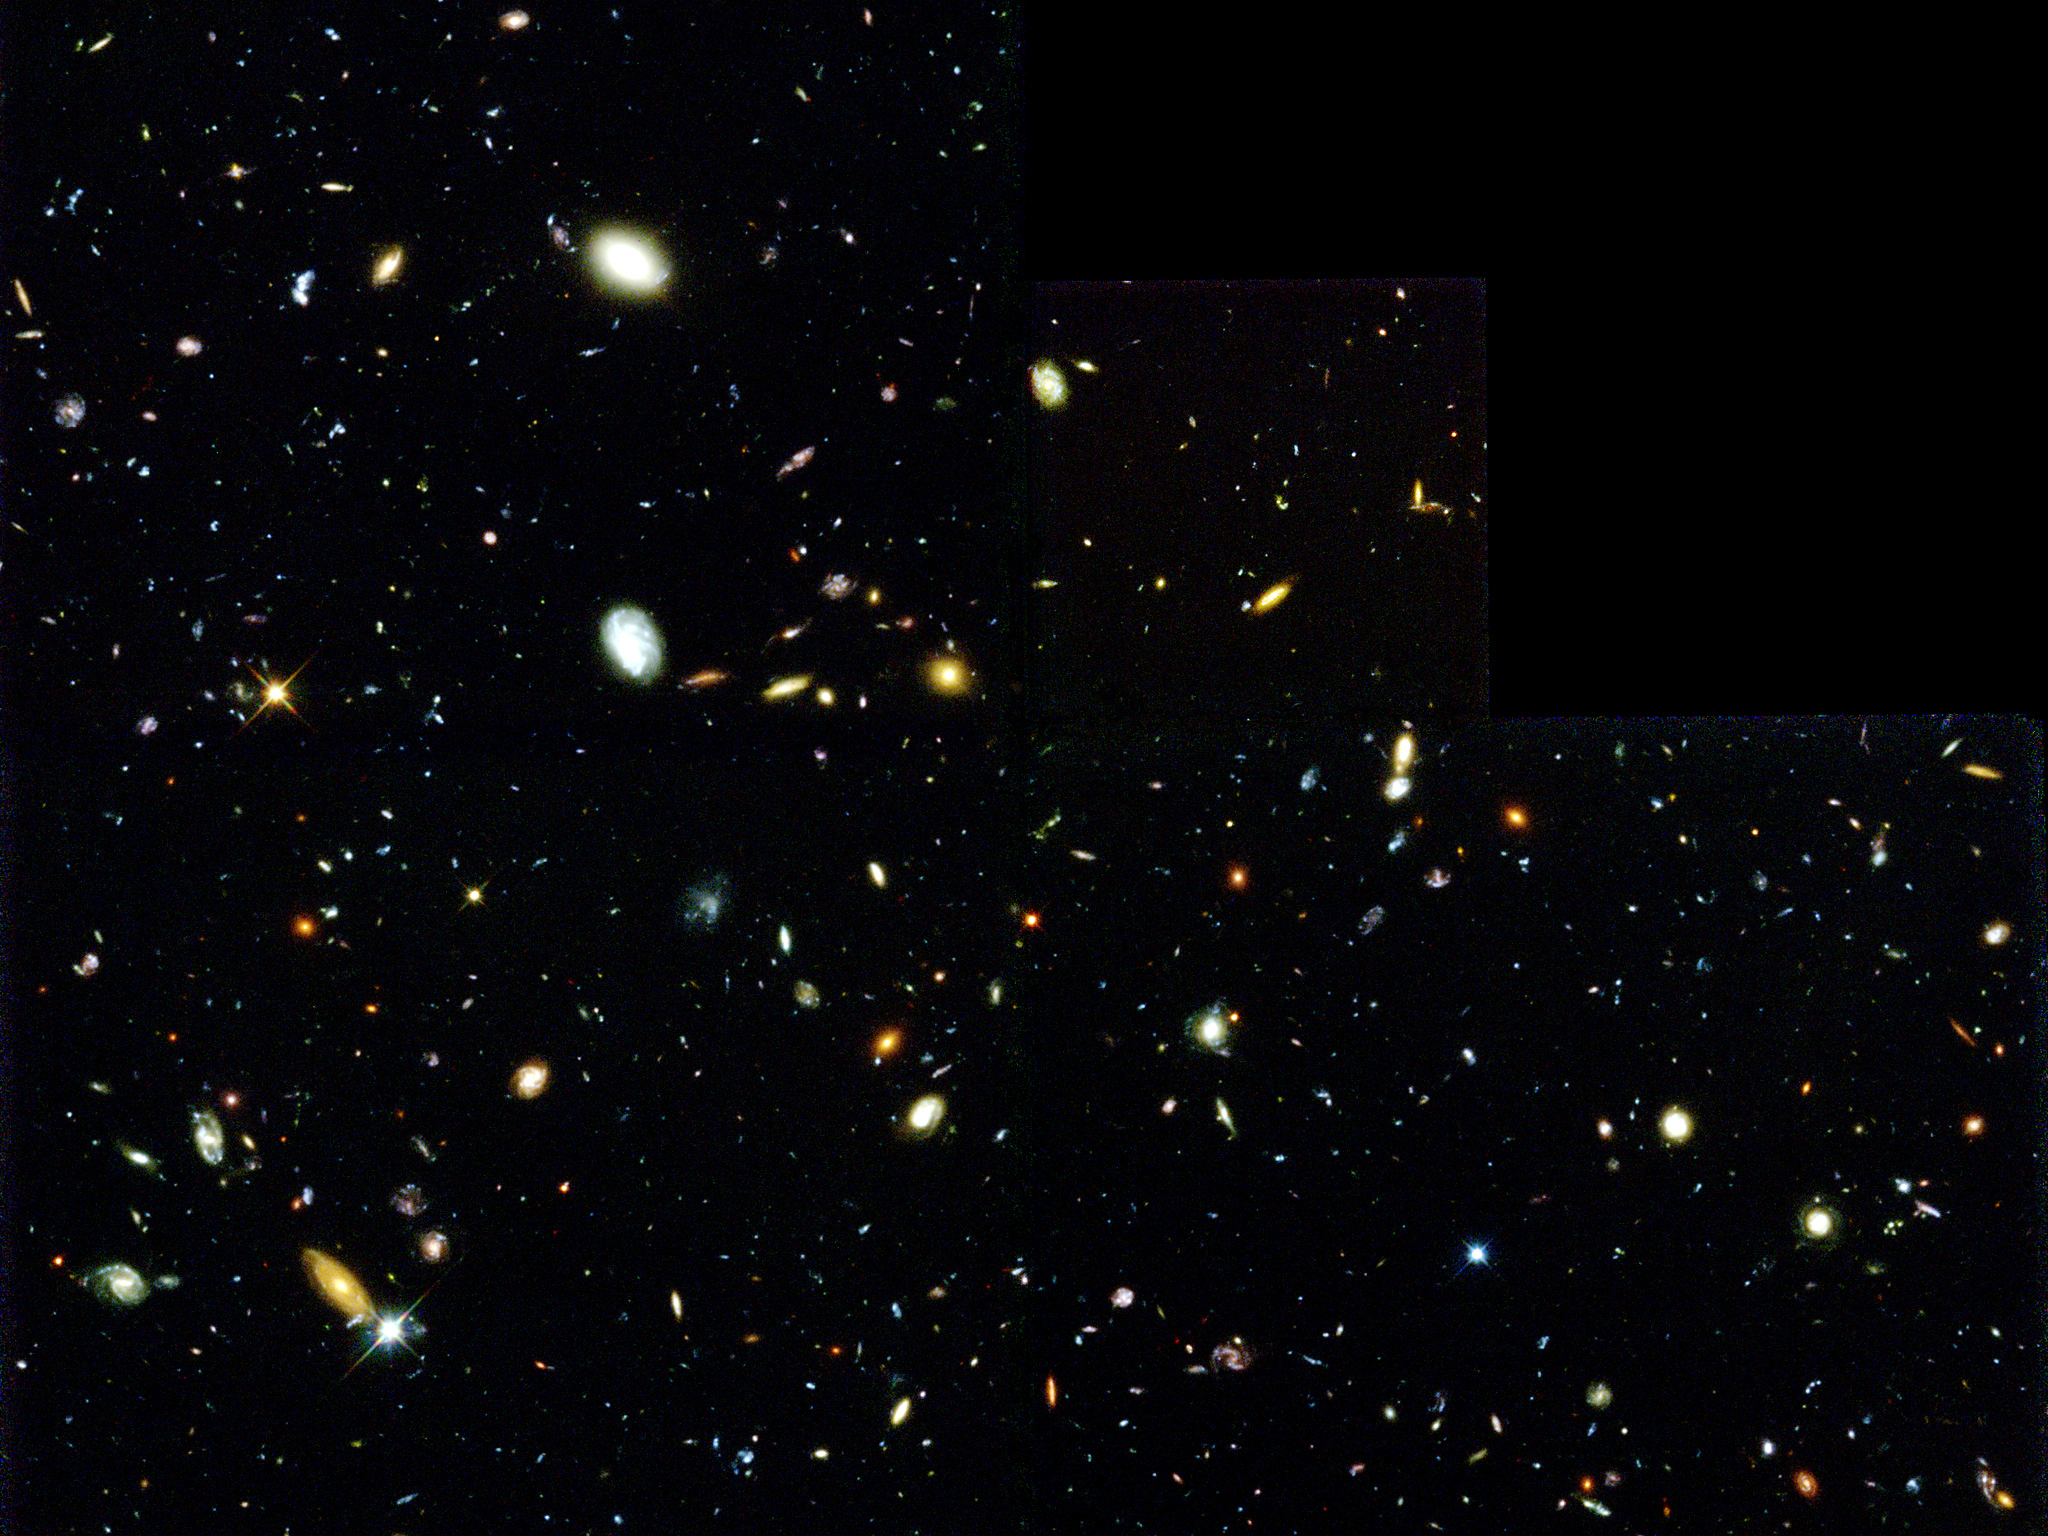
\includegraphics[width=0.9\columnwidth]{Figures/hubble_deep_field.jpeg}
	\caption{The Hubble Deep Field as captured by the Wide Field and Planetary Camera 2 onboard the \textit{Hubble Space Telescope} in 1995.}
	\label{fig:hubble_deep_field}
\end{figure}

\section{Galaxy Formation and Evolution}

To answer our questions on the evolution of galaxies, we must first make some inferences about the {\color{red}[...]} of the Universe. Our understanding of the cosmic history of galaxies is dependent on our choice of cosmology, which is widely accepted to be in the form of the $\Lambda$-CDM model (\citealt{Peebles_1980}). In the $\Lambda$-CDM model, Cold Dark Matter, matter of unknown origin, dominates over ordinary baryonic matter; and with dark energy, constitute a combined $\sim 95\%$ of the total cosmic energy budget (\citealt{Fukugita_2004}). The presence of dark matter is only evident in its gravitational interactions with other matter, but its origin is unknown as it does not interact with nor emit any electromagnetic radiation. The dark energy in the Universe is parameterized in the form of the cosmological constant, $\Lambda$, which is required to explain the accelerating expansion of the Universe. In this model, galaxy formation is seeded by small quantum fluctuations in the density of the early Universe, which grow with inflation to form small overdensities that later become the sites of dark matter halos by gravitationally attracting nearby dark matter. The first galaxies formed from these originally minute overdensities in density, which later merge due to an increase in collisions in a smaller Universe, to form ever larger galaxies. This model of galaxy formation is called a 'hierarchical' model, where galaxies in the early Universe are expected to be smaller and formed their mass more quickly than massive galaxies at later times that formed much of their stellar mass from previous mergers. As we shall show in Chapter \ref{chapter:Radio_Identifications}, this model of evolution may not explain the stellar build up of all galaxies.

\subsection{Classification of Galaxies}

The first step in understanding galaxy evolution by observing how galaxies have changed as we look back in time, is to classify galaxies according to their observable properties. Generally, galaxies can be classified into two broad groups based on their morphology: spirals and ellipticals. This dichotomy prompted the first classification scheme by Edwin Hubble (Figure \ref{fig:hubble_tuning_fork}; \citealt{Hubble_1936}), the \textit{Tuning Fork}, which shows ellitpical galaxies along the "handle", becoming more oblate towards the spiral galaxies. The spiral galaxies themselves are split into two categories forming the two "prongs", depending on the presence of a bar at the centre. At the join of the two, classified on the \textit{Tuning Fork} as S0, is where we might locate \textit{lenticular galaxies}, that are recognized by their large disks, like spirals, but without the presence of arms. In the rest of this Thesis we shall predominantly be referring to elliptical galaxies at \textit{early-type galaxies} (ETGs) and spiral-like galaxies as \textit{late-type galaxies} (LTGs), as is convention. Despite their names, the two do not represent a former and latter evolutionary stage of a typical galaxy, and is rather a misnomer. A minority of galaxies do not conform to this dichotomous image and are typically grouped together as \textit{irregular galaxies}.

\begin{figure}
    \centering
	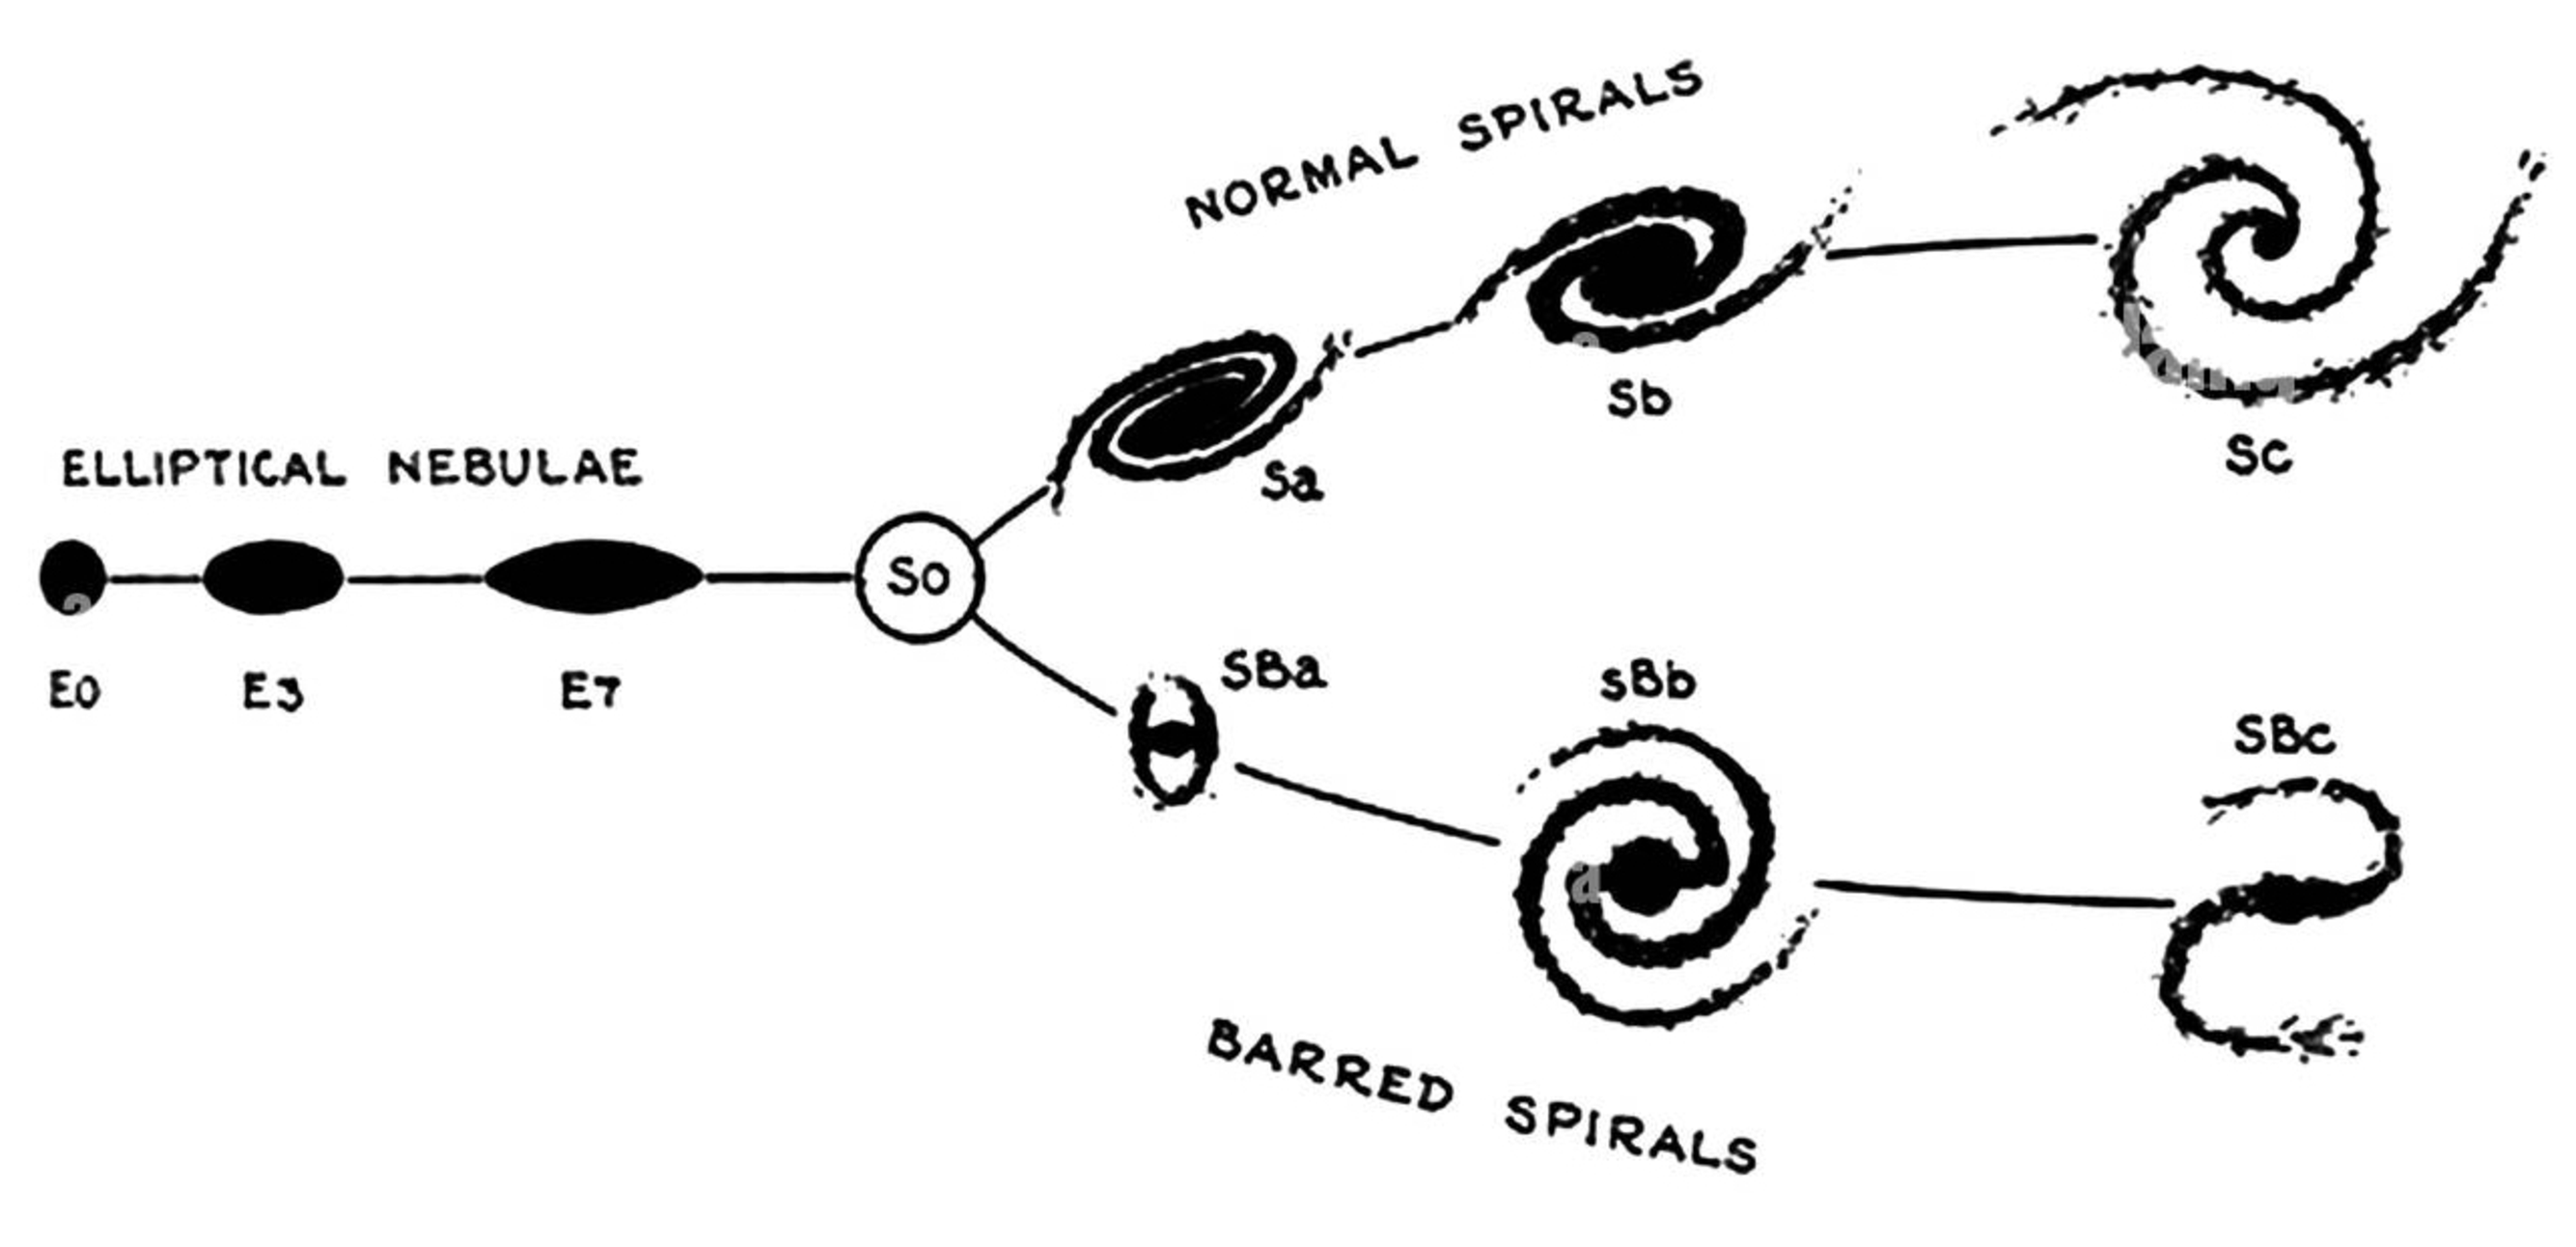
\includegraphics[width=0.9\columnwidth]{Figures/hubble_tuning_fork}
	\caption{The \textit{Hubble Tuning Fork}, or the \textit{Sequence of Nebular Types} as named in \citealt{Hubble_1936}, showing spiral galaxies along the prongs of the tuning fork and elliptical galaxies along the handle. The two prongs separate those spiral galaxies with barred central bulges from those that do not. Lenticular galaxies can be found at the join of the handle to the prongs. From left to right, the elliptical galaxies become more oblate and the spiral galaxies have spiral arms that become less tightly wound around the central bulge.}
	\label{fig:hubble_tuning_fork}
\end{figure}

Beyond their shape, the two broad groups, ETGs and LTGs, have a number of physical characteristics that are common to galaxies of the same class. First, the stellar populations of ETGs and LTGs are different. ETGs are dominated by old stellar populations that appear red in colour because they contain longer-lived, low mass stars, whereas LTGs typically have younger stellar populations of massive, but very short-lived stars.

ETGs are considered to be some of the most massive, luminous galaxies (due to having vast quantities of old stars) observed in the local Universe (\citealt{Bernardi_2003}; \citealt{Kelvin_2014}; \citealt{Moffett_2016}). Their stellar content is often centrally distributed, with the density of stars decreasing to the outskirts of the galaxy. In this central bulge of stars is where most of the interstellar medium (ISM) is located, though it is not expected to be substantial, and the limited amount of gas prohibits new star formation. In a hierarchical view of star formation, such ellipticals are formed from a series of major and minor mergers that consume the gas in the galaxy, leading to the quiescent systems observed today (\citealt{Toomre_1972}). In contrast, LTGs have dusty spiral arms with sites of active star formation, with older stars mainly located within the central bulge. While ETGs are largely devoid of gas, LTGs have a rich ISM that continues to fuel star formation, creating new stars at typical rates of several stars per year (\citealt{Kennicutt_1983}; \citealt{Gao_2004}). Our own Milky Way is an SBc spiral galaxy (\citealt{Gerhard_2002}) with active star formation at a rate of $\sim 2\,M_\odot$yr$^{-1}$ (\citealt{Noriega-Crespo_2013}; \citealt{Licquia_2015}; \citealt{Elia_2022} and references therein).

\subsection{The Star Forming Main Sequence}

A natural diagram to illustrate the difference in colour of ETGs and LTGs is to show the colours of optically-selected galaxies against their absolute magnitude. Galaxies discovered in optical surveys readily form two distinct regions: a \textit{red sequence} and a \textit{blue cloud}, with a sparsely populated region in between, the \textit{green valley}. Due to their optical colours, the red sequence is dominated by ETGs and the blue cloud dominated by LTGs. Moving away from observed quantities to intrinsic quantities, we note that the colour is a strong indicator of the star formation rate (SFR) in a galaxy and that absolute magnitude is approximately proportional to the size of the stellar population, and thus the stellar mass, $M_*$. In this formalism, the blue galaxies form a tight correlation known as the \textit{Main Sequence} (MS) or \textit{Star Forming Main Sequence}, while the red sequence occupies a \textit{passive cloud} (or "red and dead" or "quiescent") region that lies below the MS at lower star formation rates (\citealt{Noeske_2007}; \citealt{Daddi_2007}; \citealt{Elbaz_2007}; \citealt{Rodighiero_2011}). Figure \ref{fig:star_forming_main_sequence} shows the main sequence and passive clouds (grey contours) that form from the optically-selected Sloan Digital Sky Survey (SDSS; \citealt{York_2000}). \citealt{Saintonge_2017} present the \textit{Extended CO Legacy Database for GASS}, xCOLD GASS, a mass-selected sample from SDSS that have molecular gas mass estimates, which are plotted in colour in Figure \ref{fig:star_forming_main_sequence}. The molecular gas mass fraction, $f_{\textrm{H}_2} \equiv M_{\textrm{H}_2}/M_*$, clearly declines towards the passive cloud, showing the depleted ISM in ETGs.

{\color{red}Perhaps add a paragraph on the stellar-mass growth sequence, as illustrated by Figure 12 of Graham+2023}

\begin{figure}
    \centering
	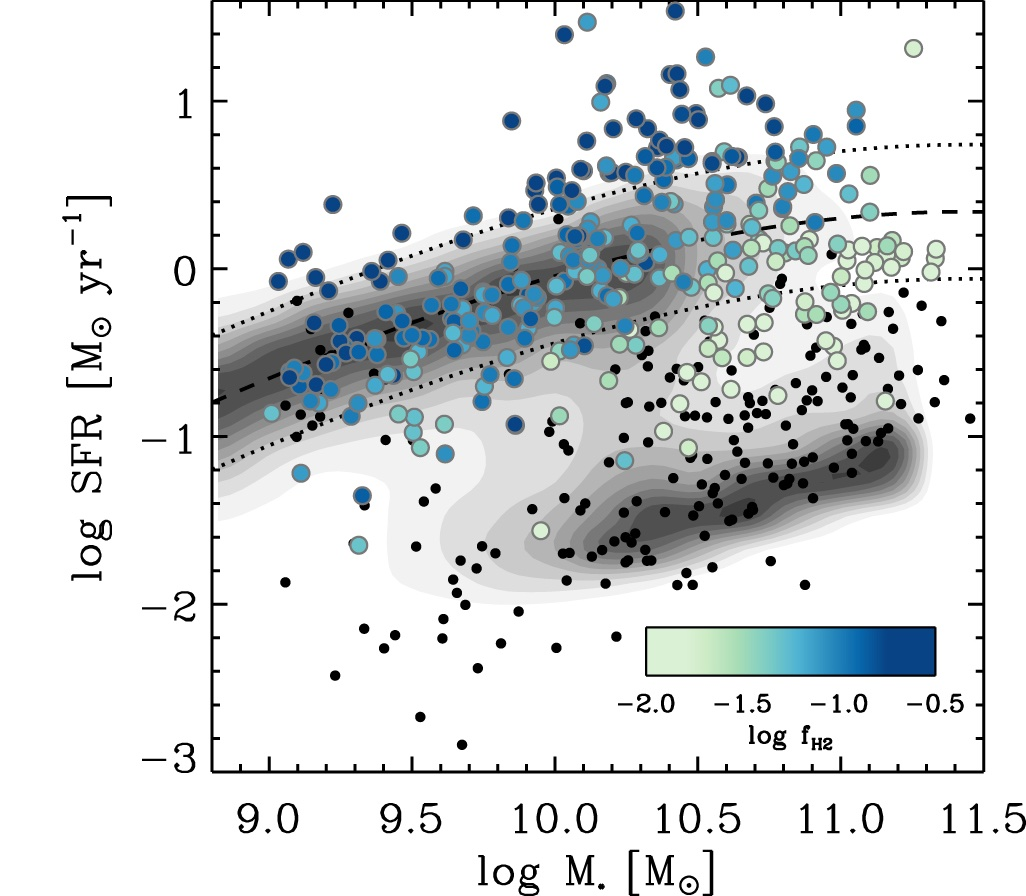
\includegraphics[width=0.75\columnwidth]{Figures/saintonge_ms.jpg}
	\caption{The distribution of SDSS galaxies in the SFR-$M_*$ plane (grey contours) from \citealt{Saintonge_2017} (Figure 7). The dashed line represents the location of the main sequence, while the dotted lines represent $\pm0.4\,$dex scatter around this relation. The coloured points show the distribution of galaxies from xCOLD GASS, coloured according to their molecular gas mass fraction.}
	\label{fig:star_forming_main_sequence}
\end{figure}

It is predicted that the vast majority, approximately $90\%$, of all cosmic star formation between redshifts $0$ and $2.5$ occurs in galaxies that reside on the MS, however, an important contribution also comes from galaxies that sit substantially above the relation. These galaxies, undergoing high levels of star formation for a short period of time, are collectively referred to as \textit{starburst galaxies} (e.g. \citealt{Muxlow_2006}; \citealt{Rinaldi_2022}). Starbursts form a small minority of galaxies, approximately $2\%$ of star forming galaxies depending on the exact definition of a starburst, but contribute $\sim 10\%$ of the cosmic star formation rate density (SFRD) at $z \sim 2$ (\citealt{Rodighiero_2011}), corresponding to the time in cosmic history when star formation was at its peak (see Section \ref{sec:cosmic_star_formation_history}).

Given that galaxies in the passive cloud have large stellar masses, they must have been at some point among the actively star forming galaxies, and then some process quench them of their star formation leading them to the passive cloud. The prevailing interpretation of the SFR-$M_*$ diagram is that a typical galaxy evolves along the sequence, gaining stellar mass, increasing their star formation rate accordingly and depleting the gas available for star formation in the process. At some point, the galaxy stops forming stars entirely, and falls off the main sequence. The valley between the MS and the passive cloud, a result of a dearth of galaxies in this regime, suggests that the quenching process that turns off the star formation in the galaxy is fast. This image of galaxy evolution, however, is not without scepticism. Recent studies (e.g. \citealt{Eales_2018}; \citealt{Bremer_2018}; \citealt{Phillipps_2019}) have suggested that the bimodal distribution of star forming and passive galaxies may be a reflection of selection effects in optical surveys, prompting attempts to define the whole population of galaxies using a probability distribution with only one maximum (e.g. \citealt{Corcho-Caballero_2020}). {\color{red}Explain the evidence for an apparent bimodality (Read abstracts of three papers above - that is all that is needed.)}

Whether there are two distinct classes or whether the transition between morphological types and physical properties is gradual, some physical process must be coverting a star forming galaxy on the MS to one that is passive, quenching it of star formation. There are many possibilities that have been proposed as the cause of quenching, and it is likely that all are important in different scenarios. These processes include stellar feedback and winds from supernovae removing the gas from a galaxy (\citealt{Hayward_2017}); gas expulsion by active galactic nuclei, AGN (\citealt{Springel_2005}; \citealt{Croton_2006}; \citealt{Cicone_2014}; \citealt{Harrison_2017}); the formation of a galactic bar or central bulge (\citealt{Bournaud_2007}; \citealt{Martig_2009}) which relocates the gas to the galactic center and reduces the star formation in the disk, as well as a range of environmental processes such as galaxy merging (\citealt{Lavery_1994}; \citealt{Weigel_2017}) which ignites a starbursting phase that rapidly consumes the gas; ram-pressure stripping, the loss of gas as the galaxy passes through the intra-cluster medium (\citealt{Gunn_1972}; \citealt{Boselli_2006}; \citealt{Domainko_2006}; \citealt{Boselli_2014}), and quenching mechanisms that result from being in high density environments such as galaxy clusters, like galaxy harassment and strangulation (\citealt{Moore_1996}; \citealt{Moore_1998}; \citealt{Bekki_2002}).

\subsection{Cosmic Star Formation History}
\label{sec:cosmic_star_formation_history}

We have seen that the star formation rates of galaxies is intrinsically linked to its evolutionary stage, and thus it would be unsurprising to identify an evolution in the integrated SFRs of galaxies with cosmic time. By measuring the star formation of many galaxies at different epochs, we can build a picture of the star formation density in the Universe. The cosmic history of star formation is one of the fundamental observables of astronomy, giving us an insight into the timeline for which gas forms into stars, heavy elements are produced (elements heavier than the primordial hydrogen and helium are produced in stars), and dust is formed (as dust is a natural byproduct of star formation, see Section {\color{red}X}).

The cosmic star formation rate density (SFRD {\color{red}Repeated}) in the Universe can be estimated in two ways. The most straightforward way to estimate the star formation rate is to measure the amount of starlight we observe from tracers of recent star formation in galaxies. In this sense, the SFR indicator should be sensitive to the short-lived massive stars at each point in cosmic history, and thus the UV and optical stellar light is often used (e.g. \citealt{Madau_1996}; \citealt{Lilly_1996}; \citealt{Wyder_2005}; \citealt{Schiminovich_2005}; \citealt{Dahlen_2007}; \citealt{Reddy_2009}; \citealt{Robotham_2011}; \citealt{Cucciati_2012}; \citealt{Schenker_2013}; \citealt{Finkelstein_2015}). Second, we note that approximately half of all optical and UV light from stars ever emitted in the Universe has been absorbed by dust and re-emitted at far-infrared (FIR) and sub-millimeter (sub-mm) wavelengths (\citealt{Puget_1996}; \citealt{Fixsen_1998}; \citealt{Dole_2006}; \citealt{Driver_2008}; \citealt{Driver_2016}). This means that a significant contribution to the SFRD must also be measured from far-IR/sub-mm indicators of star formation that probe the stellar light reprocessed by dust (e.g. \citealt{Magnelli_2011}; \citealt{Casey_2012}; \citealt{Magnelli_2013}; \citealt{Gruppioni_2013}; \citealt{Swinbank_2014}; \citealt{Bouwens_2016}; \citealt{Bourne_2017}; \citealt{Koprowski_2017}; \citealt{Novak_2017}; \citealt{Liu_2018}; \citealt{Bouwens_2020}; \citealt{Dudzeviciute_2020}).

{\color{red}Rewrite above as it is not strictly two separate ways. See Wise+2023.}

Figure \ref{fig:cosmic_sfrd} shows that the dust-obscured and unobscured measures of the SFRD have peaks at $z\sim2$ (when the Universe was roughly 3 billion years old), followed by a slow decline by a factor of $\sim 8$ to the present day. The short period corresponding to the peak of star formation is often referred to as \textit{cosmic noon}. In the (approximate) 3.5\,Gyr between $z\sim3$ and $z\sim1$, spanning cosmic noon, up to half of the stellar mass we observe today was formed (\citealt{Forster-Schreiber_2020}). The galaxies that are identified at these redshifts are ideal targets for tracing the formational epoch of the massive LTGs and ETGs seen in the local Universe. We see that most of the star formation at $z < 3$ is obscured by dust and even at higher redshifts the contribution appears significant. The FIR and sub-mm traced component has dominated the cosmic history of star formation for the past $\sim 12\,$Gyr, contributing approximately $80\%$ of the total star formation. The top panel of Figure \ref{fig:cosmic_sfrd} shows the contribution from galaxies with different IR luminosities to the dust-obscured star formation. It is clear that massive, IR luminous galaxies dominate the star formation history at earlier times. At this point, we clarify some acronynms commonly used to refer to bright infrared galaxies (the IR luminosities of galaxies are assumed to be the bolometric luminosity integrated between $8$ and $1,000\,\mu$m):

\begin{itemize}
    \item Luminous Infrared Galaxy (LIRG) - Defined as having $10^{11} < L_\textrm{IR} [L_\odot] < 10^{12}$.
    \item UltraLuminous Infrared Galaxy (ULIRG) - Defined as having $10^{12} < L_\textrm{IR} [L_\odot] < 10^{13}$.
    \item HyperLuminous Infrared Galaxy (HyLIRG) - Defined as having $L_\textrm{IR} [L_\odot] > 10^{13}$.
\end{itemize}

\begin{figure}
    \centering
	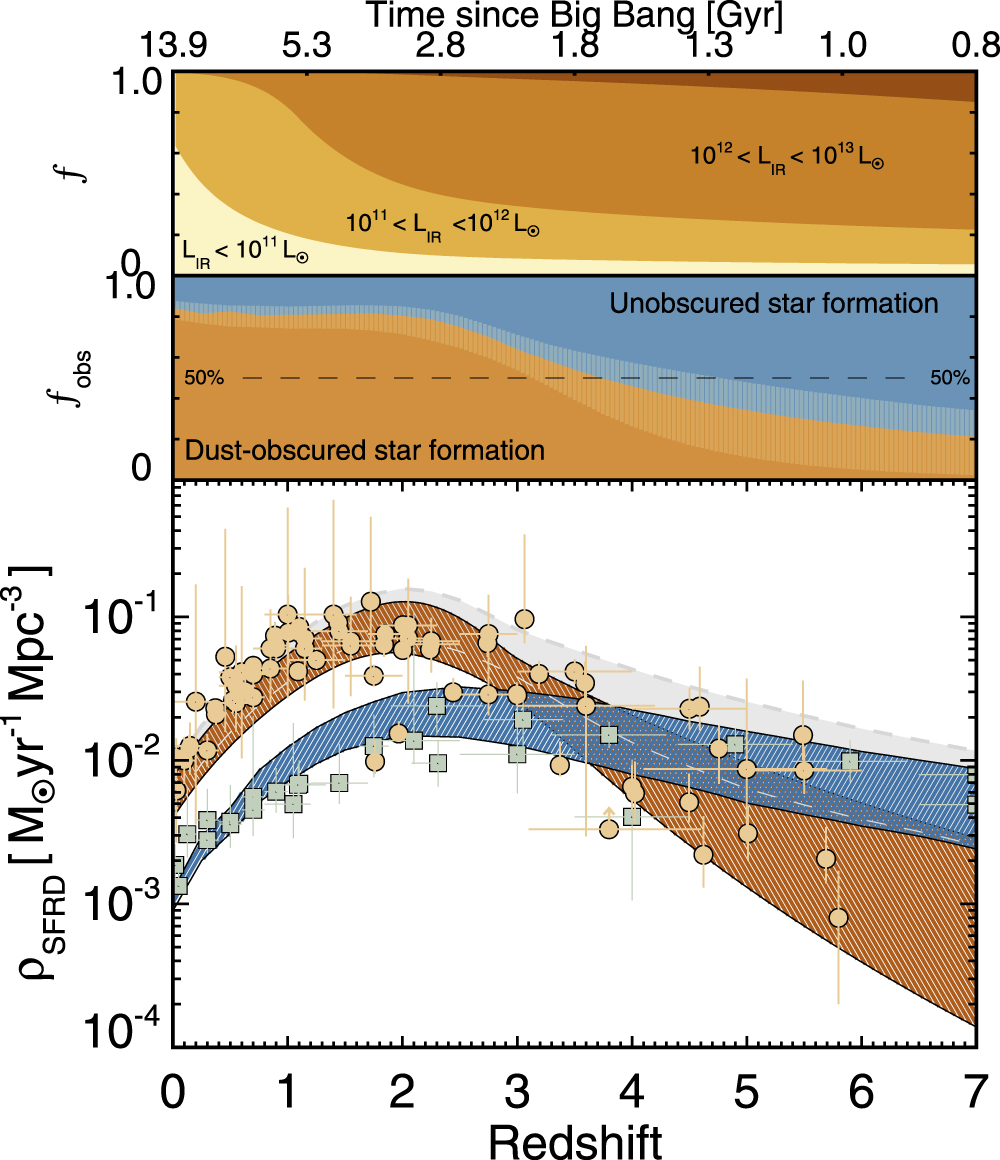
\includegraphics[width=0.75\columnwidth]{Figures/cosmic_sfrd.jpeg}
	\caption{The cosmic star formation history from \citealt{Zavala_2021}. The contributions to the total star formation rate density (grey) from dust-obscured IR/sub-mm surveys and from unobscured UV/optical surveys are shown in orange and blue, respectively. The top panel shows the contribution from galaxies with different IR luminosities to the dust-obscured SFRD. The classes shown are $L_\textrm{IR} < 10^{11}\,L_\odot$, $10^{11} < L_\textrm{IR} [L_\odot] < 10^{12}$ (LIRGs) and $10^{12} < L_\textrm{IR} [L_\odot] < 10^{13}$ (ULIRGs). The middle panel represents the fraction of SFRD that is dust-obscured.}
	\label{fig:cosmic_sfrd}
\end{figure}

Looking back to cosmic noon, much of the star formation within dusty galaxies is happening in ULIRGs, while the integrated dust-obscured star formation begins to fall. This suggests that the number of massive galaxies declines at higher redshifts. Particularly at high redshifts ($z \gtrsim 3$), the exact amount of dust-obscured star formation is still uncertain. Large samples of galaxies with measured dust emssion are therefore required to elucidate our view on the cosmic history of star formation.

\section{The Interstellar Medium}

The interstellar medium (ISM) refers to the matter that fills the space in between the stars of a galaxy. It is the medium in which stars are born, and latter replenished with enriched material when they die. The matter comes in the form of gas - in ionic, atomic and molecular forms - and dust, in overwhelming favour of gas which constitutes $\sim99\%$ of the ISM, and dust the other $1\%$ ({\color{red}REFERENCE}). By mass, the gas in the ISM is around $70\%$ hydrogen, $28\%$ helium and $2\%$ heavier elements, reflecting only a small change from the ratios of the primordial matter created after the Big Bang (\citealt{Klessen_2016}). In terms of volume, most of the ISM is occupied by ionized gas, but due to its incredibly low volume density, only accounts for around $25\%$ of the gas mass. Most of the gas mass in a galaxy is in the form of neutral atomic gas (H and He) or molecular (H$_2$) and can be found in dense clouds that take up only $1-2\%$ of the total volume of the ISM.

The ISM spans a wide range of temperatures and densities, leading to many interpretations of the ISM as being in distinct phases, despite there being no obvious separation between different phases (\citealt{Cox_2005}). A two phase model was proposed by \citealt{Field_1969}, showing that atomic gas in the ISM can exist at two stable temperatures. These two solutions correspond to cold and dense gas at $T\sim100\,$K and warm, diffuse gas at $T\sim10^4\,$K. These are now referred to as the Cold Neutral Medium (CNM) and Warm Neutral Medium (WNM), respectively. This model was extended to three phases by \citealt{McKee_1977}, who noted that supernovae in the ISM creates bubbles of very hot, ionized gas ($T\sim10^6\,$K). This phase of the ISM is known as the Hot Ionized Medium (HIM). A cooler, Warm Ionized Medium (WIM) has a temperature and density similar to the WNM, but contains around $90\%$ of the ionized gas in the ISM (\citealt{Haffner_2009}). A final distinction is typically made for the molecular clouds that are cold, but distinctly more dense than the CNM. The molecular gas clouds have a range of masses and sizes, and is known to correlate with observed star formation in the Galaxy. The approximate temperatures, densities, mass fractions and volume filling fractions of the phases in the ISM for a dynamic spiral galaxy is given in Table \ref{tab:ISM_phases} as presented in \citealt{Ferriere_2001} and {\color{red}Walter?}. The fractions are highly uncertain but represent what might be realistic estimates for a spiral galaxy containing all five phases of this model of the ISM.

\begin{table}
	\centering
	\begin{tabular}{p{4cm}|p{3cm}|p{3cm}|p{1.5cm}|p{1.5cm}}
		\hline
		\hline
		Phase & T [K] & $n$ [atoms cm$^{-3}$] & $f_{\textrm{Mass}}$ & $f_{\textrm{Volume}}$ \\
		\hline
		\hline
		Molecular Clouds & $10 - 20$ & $>10^2$ & $\sim 20\%$ & $<1\%$ \\
		Cold Neutral Medium & $50 - 100$ & $20 - 50$ & $\sim 40\%$ & $\sim2 - 4 \%$\\
		Warm Neutral Medium & $6,000 - 10,000$ & $0.2 - 0.5$ & $\sim 30\%$ & $\gtrsim 30\%$ \\
		Warm Ionized Medium & $\sim8,000$ & $0.2 - 0.5$ & $\sim 10\%$ & $\gtrsim 15\%$ \\
		Hot Ionized Medium & $\sim10^6$ & $\sim10^{-2}$ & $\sim 1\%$ & $\lesssim 50\%$ \\
		\hline
	\end{tabular}
	\caption{The different phases of the ISM and their expected temperatures, densities, mass fractions and volume filling factors.}
	\label{tab:ISM_phases}
\end{table}

This multi-phase picture is certainly an oversimplification of the conditions found in the ISM. The ISM is shaped by a variety of processes that blur the distinction between these distinct phases. The actual ISM is continuous and dynamic with transitional regions between the phases. Processes that contribute to the blurring of the boundaries between different phases include turbulence from supernova shocks (\citealt{MacLow_2004}) and stellar winds, thermal instability (\citealt{Kritsuk_2002}) and the presence of magnetic fields.

Figure \ref{fig:interstellar_medium} shows various components of the ISM in the Galaxy, as traced by different wavelengths of the electromagnetic spectrum. The top two panels highlight the starlight that is observable at optical ($0.5\,\mu$m) and near-infrared ($2\,\mu$m) wavelengths. The stellar light is blocked by dust in the optical image, whereas the near-infrared clearly shows the stellar distribution, making the dark dust clouds appear almost transparent. The benefit that the infrared provides in identifying the stellar light of a galaxy, compared to optical wavelengths, is a key motive for the studies presented in Chapters \ref{chapter:Data_Release_3} and \ref{chapter:Dust_Mass_Functions}. As we traverse the electromagnetic spectrum to the far-infrared (third panel, observed at $350\,\mu$m) the emission from the dust itself becomes visible. The final three panels show the emission from atomic, ionized and molecular gas in the Galaxy. The atomic gas is traced by the $21\,$cm spectral line, originating from the hydrogen \textit{spin-flip} transition between a proton-electron aligned state to an anti-aligned state. This transition is forbidden - the mean lifetime of a hydrogen atom being in the excited, aligned state is approximately 11 million years ({\color{red}REFERENCE}) - meaning that the likelihood of the transition is incredibly rare. However, as can be seen in the figure, the abundance of atomic hydrogen means that the $21\,$cm line is a useful tracer for gas in the ISM. The limitation of the $21\,$cm line is that it is only useful for tracing the distribution of neutral hydrogen in the local Universe where the emission is still strong enough to be detected. The $74\,$cm radio emission in the penultimate panel traces the radiation from ionized gas. The radio emission emanates from accelerated charged particles, which may be observed in HII regions and supernova remnants. The final panel shows the molecular gas phase, as traced by the $2.6\,$mm spectral line of carbon monoxide (CO). As will be detailed later, the rotational transitions of the CO molecule is a useful tracer of dense molecular regions, and it is often assumed that wherever there are CO molecules there must also exist H$_2$ molecules. This map shows the locations of cold gas in the Galaxy and the sites of star formation.

\begin{figure}
    \centering
	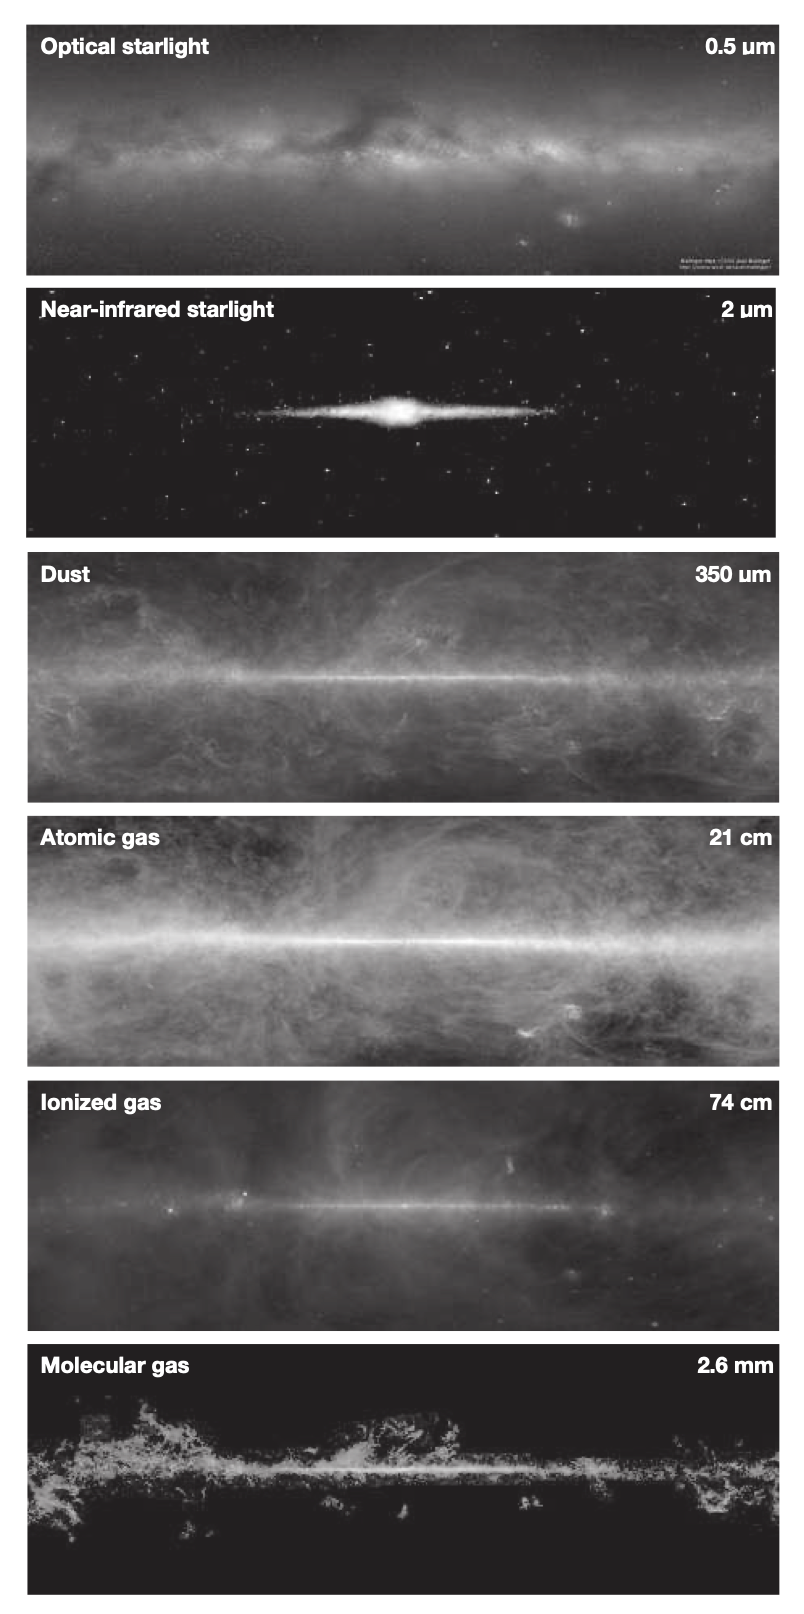
\includegraphics[width=0.75\columnwidth]{Figures/interstellar_medium.png}
	\caption{{\color{red}Caption.} \citealt{Williams_2021}}
	\label{fig:interstellar_medium}
\end{figure}

A fundamental assumption that is made throughout this Thesis is that we can trace the hidden star formation in a galaxy via the dust emission observed in the far-IR and sub-mm wavelengths (as discussed in the following section). Figure \ref{fig:interstellar_medium} shows that the dust and gas are well mixed in the ISM of the Galaxy, and in Section \ref{sec:dust_tracing_star_formation} we describe how dust is an integral part of the star formation process in galaxies. As such, this assumption appears to hold and we may study the dust content of galaxies, and make inferences about their star formation, from the radiation emitted at far-IR and sub-mm wavelengths.

\section{Cosmic Dust}

\subsection{Chemical Composition and the Reprocessing of Starlight}

Cosmic dust is a general term that refers to the solid particles that exist in the ISM. These interstellar grains can have a range of sizes between $\sim 10\,$nm and $\sim 1\,\mu$m (\citealt{Kim_1994}; \citealt{Galliano_2018}) and are mostly composed of carbonaceous materials (materials that are predominantly Carbon by mass) and silicates. The larger dust grains are primarily silicates and amorphous carbon, which are the prime candidates for the dust grains that absorb UV and optical starlight and reradiates this energy in the far-IR and sub-mm regimes. Hydrogenated carbonaceous materials, like Polycyclic Aromatic Hydrocarbons (PAHs), are chemical compounds comprised of carbon and hydrogen molecules and are also {\color{red}[...]} interstellar dust grains. These molecules are the cause of strong spectral lines that can be observed in the mid-infrared (\citealt{Tielens_1987}; \citealt{Draine_2007a}; \citealt{Draine_2007b}).

The presence of dust along the line of sight to a population of stars can have several consequences on the emission that is observed. First, if the dust is thick enough, any background stellar light may not be visible at all, as is the case with some dark nebulae in the Galaxy such as the \textit{Horsehead Nebula}. For less opaque dust clouds, the light passing through can be dimmed due to the effects of dust extinction. This refers to the amount of background light that is absorbed and scattered out of the line of sight to the observer. The dimming effect is dependent on several factors including the density of the dust cloud, the grain size distribution and the wavelength of the light. More generally, dust attenuation refers to the effect on the spectrum of a background object as a result of dust, which includes dust extinction, but also includes scattering back into the line of sight and the light from unobscured stars. It is the attenuated stellar emission that is observed as a strong peak in the far-IR region of a galaxy's spectral energy distribution (SED). Figure \ref{fig:unattenuated_attenuated_sed} shows the UV to far-IR SED of NGC337, modelled using \texttt{MAGPHYS} (\citealt{daCunha_2008}), which illustrates how the true stellar spectrum of a galaxy (blue) is attenuated by dust to produce the far-IR emission (green) and the observed UV to far-IR spectrum (black). Moreover, interstellar dust is more efficient at absorbing and scattering blue light compared to red light, meaning that background stars behind a cloud of dust often appear more red than they are. This effect is known as interstellar reddening and can be observed in the spectrum of NGC337 - the shorter the wavelength (towards the blue end of the spectrum), the greater the difference between the attenuated and unattenuated stellar spectra.

\begin{figure}
    \centering
	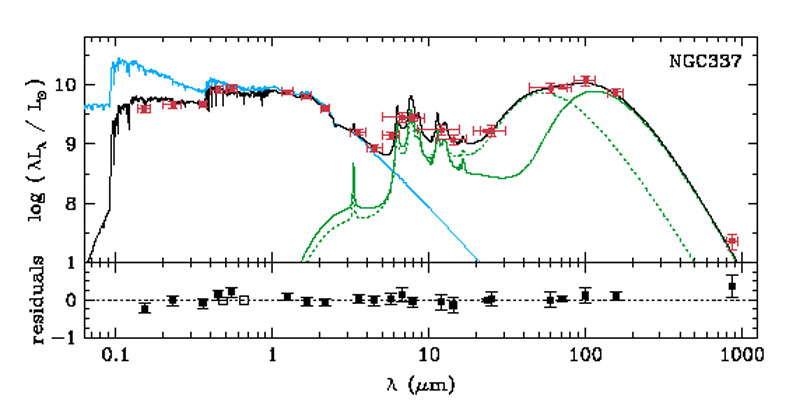
\includegraphics[width=0.9\columnwidth]{Figures/unattenuated_attenuated_sed.jpeg}
	\caption{{\color{red}Caption.} \citealt{daCunha_2008}}
	\label{fig:unattenuated_attenuated_sed}
\end{figure}

\subsection{The Lifecycle of Dust}

The lifecycle of dust grains, the mechanisms in which they are produced and destroyed, are important in understanding the metal enrichment and stellar evolution of galaxies. Dust can form in a number of ways including in the stellar winds of evolved stars, from the ejecta of supernovae or they can form in situ in the ISM (\citealt{Draine_2009}). Traditionally, the majority of dust was presumed to be formed in the outer envelopes of latter stage stars, such as red giant branch (RGB) and asymptotic giant branch (AGB) stars. These stars have masses of $1 < M_\textrm{star} [M_\odot] < 8$ and are in a late phase of evolution, having left the (stellar) main sequence and formed heavy elements. The metals solidify into grains in the envelopes of RGB and AGB stars and are carried out in the stellar wind and deposited into the ISM ({\color{red}REFERENCE}). For more massive stars with $M_\textrm{star} > 8\,M_\odot$, dust can form in the ejecta of {\color{red}[...]} supernovae, condensing from the leftover expanding material. The problem with this pathway, however, is that the dust yields from a single supernova are still a matter of debate, with studies observing dust masses in supernova remnants between roughly $0.05\,M_\odot$ and $1\,M_\odot$ (\citealt{Rho_2008}; \citealt{Dunne_2009}; \citealt{Barlow_2010}; \citealt{Matsuura_2011}; \citealt{Gomez_2012}; \citealt{Matsuura_2015}; \citealt{Chawner_2019}). Much of this debate is due to questions about how dust formed in supernovae may survive the destructive shock waves that are produced (\citealt{Draine_1979}; \citealt{Jones_1996}). The production rate of dust is a key open question, particularly for studies in the early Universe where a \textit{Dust Budget Crisis} has been proposed (e.g. \citealt{Dwek_2007}; \citealt{Michalowski_2010}; \citealt{Valiante_2011}). This refers to the difficulty in explaining the high dust masses observed in high redshift galaxies from dust produced via the Low-Intermediate Mass Stars (LIMS). Above redshifts $\sim 5$, there is little time for significant amounts of dust to be produced from the post main-sequence evolution of LIMS (\citealt{Morgan_2003}; \citealt{DiCriscienzo_2013}). The final production mechanism we mention here is dust formed in situ via grain growth. This method is most effective in the dense ISM, and so is particularly important in molecular clouds. Grain growth occurs when the conditions allow for the grains to form mantles of ice, which allow metals to subsequently stick to the grains (coagulation, \citealt{Blain_2004}).

We have mentioned one way in which dust can be destoyed in the ISM, via supernova shocks, but a second process contributing to dust destruction is \textit{sputtering}. Sputtering occurs as the result of the bombardment of gas atoms in dense environments causing the sublimation of the dust grains (\citealt{Barlow_1978}; \citealt{Jones_2004}).

\subsection{Dust Emission as a Tracer of Obscured Star Formation}
\label{sec:dust_tracing_star_formation}

Despite accounting for only $1\%$ of the ISM, interstellar dust plays an important role in the processes that govern the formation and evolution of galaxies.

{\color{red}I don't know what to write here: i) Sites of H2 formation?}

\section{Observing Dusty Star Forming Galaxies in the Far-IR and Sub-mm}

It is at this point that we find it useful to define approximate boundaries between different wavelength regimes of interest when talking about dust emission.{\color{red}[...]}

The majority of the dust in the ISM by mass has temperatures of roughly {\color{red} $X - X\,$K} ({\color{red}REFERENCES}). It is the thermal emission from this cool dust that we observe in the far-IR and sub-mm regimes. As can be seen in the example SED of Figure \ref{fig:unattenuated_attenuated_sed}, the dust emission creates a steep sub-mm spectrum. 

[Observations in this regime probe most of the dust in the ISM]



\chapter{Herschel-ATLAS Data Release III}
\label{chapter:Data_Release_3}
[...]\todo[color=red]{A brief introduction to the chapter.}

\section{The Herschel-ATLAS}
\label{sec:The Herschel-ATLAS}

The \textit{Herschel} Astrophysical Terahertz Large Area Survey (H-ATLAS; \citealt{Eales_2010}) was the largest open-time sub-mm survey carried out with \textit{Herschel}. The survey was observed across five photometric bands using two instruments onboard the \textit{Herschel Space Observatory}: the Photodetector Array Camera (PACS, \citealt{Poglitsch_2010}) at 100 and 160\,\micron, and the Spectral and Photometric Imaging Receiver (SPIRE, \citealt{Griffin_2010}) at 250, 350 and 500\,\micron. Compared to the first SMGs detected using SCUBA at 850\,\micron (\citealt{Smail_1997}; \citealt{Barger_1998}; \citealt{Hughes_1998}), the PACS and SPIRE wavebands span the peak of the infrared spectrum for low redshift (z < 1) galaxies. Their intrinsic brightness at the SPIRE wavelengths makes their detection in the thousands more achievable. The main scientific goal of the survey was to estimate the dust masses and dust obscured star formation rates for thousands of nearby galaxies over a large area of sky. While the intention was for a shallow survey, the surprising sensitivity of \textit{Herschel} and the negative k-correction observed at the operating wavelengths of the SPIRE instrument (\citealt{Blain_1993}) means that many sources were observed at higher redshifts, with a median of z $\sim$ 1. The catalogues of the survey, as detailed below, includes sources with redshifts up to $\sim$ 6 (\citealt{Amblard_2010}; \citealt{Lapi_2011}; \citealt{Fudamoto_2017}; \citealt{Zavala_2018}).

The complete survey covers $\sim$\,660\,$\deg^2$, split into three regions located to avoid emission from Galactic dust and to utilize complimentary spectroscopic surveys including the Sloan Digital Sky Survey (SDSS, \citealt{York_2000}), the 2df Galaxy Redshift Survey (2dfGRS, \citealt{Colless_2001}) and the Galaxy and Mass Assembly (GAMA, \citealt{Driver_2009}). The North Galactic Pole (NGP) region covers $\sim$\,180\,$\deg^2$ of the northern sky, centered at R.A 13$^{h}$18$^{m}$ and declination +29$^{\circ}$13' (J2000); three equatorial fields, located at approximately R.A 9$^{h}$, 12$^{h}$ and 15$^{h}$ coinciding with the GAMA survey (henceforth named GAMA9, GAMA12 and GAMA15 fields), each with an area of approximately 54\,$\deg^2$, and the South Galactic Pole (SGP) region, centered at R.A 0$^{h}$6$^{m}$ and declination -32$^{\circ}$44' (J2000) with an area of $\sim$ 318\,$\deg^2$. 

\subsection{Detecting Submillimeter Sources on Herschel Images}
\label{sec:Detecting Submillimeter Sources on Herschel Images}

Due to [...]\todo[color=orange]{continuation:} sub-mm images suffer from two types of noise; instrumental noise [...]\todo[color=orange]{continuation:} and confusion noise which is highly correlated between pixels, most of its contribution coming from the blending together of faint sources. Source confusion is of particular importance to sub-mm surveys [...]\todo[color=orange]{continuation:}. The result of combining instrumental noise with confusion noise is that almost all sources in the Herschel images are unresolved and the optimum filter for detecting these unresolved sources is no longer the point spread function (PSF). Consider a \textit{Herschel} map in which there is only one source of noise: an image with instrumental noise but no confusion noise (i.e. there is only one point source and no fainter, confusing sources), the optimal detection of this source is obtained by convolving the image with the PSF of the instrument. On the other hand, a map with no instrumental noise, but many confused point sources would be optimally detected with its best signal to noise ratio (SNR) by taking the Fourier transform of the image, dividing by the Fourier transform of the PSF and taking the inverse Fourier transform to obtain a perfect deconvolution of the original map (\citealt{Valiante_2016}). For images that have a variable ratio of instrumental to confusion noise like the \textit{Herschel} images of H-ATLAS, \citealt{Chapin_2011} showed that a convolving function or "matched filter" can be calculated to provide the maximum SNR for an unresolved source.

To detect H-ATLAS sources from the 250\,\micron maps using a matched filter (the 250\,\micron band is the most sensitive of the SPIRE bands and given the lower sensitivity of the PACS instrument, all sources detected on the PACS images would also be detected on the SPIRE 250\,\micron image), \citealt{Maddox_2020} developed a source detection algorithm called the Multi-band Algorithm for Source Detection and eXtraction (MADX). The MADX algorithm works in the following way. Firstly, Galactic dust emission is removed from the images using \texttt{Nebuliser}. Next, the images are convolved with the matched filter [...]\todo[color=yellow]{continuation: description of matched filters}. The variance map is created by convolving the map of variance in instrumental noise with the matched filter and adding the confusion noise. It is from this map that the SNR of a detected source is determined. The same process is repeated with the 350 and 500\,\micron maps and interpolated to the same pixel scale as the 250\,\micron maps. The detection map used to extract sources is then generated from a weighted sum of the three SPIRE maps, however, due to the smaller PSF at 250\,\micron which leads to more accurate positions and the increased number of sources when using the 250\,\micron maps, zero weighting is given to the 350 and 500\,\micron images. This has the effect of making the detection map the same as the 250\micron map.

Sources are identified by peak values > 2.5$\sigma$ in the filtered detection map. Their positions are estimated by fitting a Gaussian to the nearest pixels surrounding the location of the peak. The source is extracted in the other \textit{Herschel} wavebands at the 250\,\micron position. Due to the high levels of confusion and high source density on the SPIRE maps, the flux density estimates in each band can be biased by blending with other sources. The MADX algorithm negates some of this problem by ordering the sources by their flux density estimates and iteratively fitting and removing a point source from the position of each source, starting with the brightest. The new estimates of the flux densities are then not influenced by contamination from brighter sources.

The catalogue of point sources provided by H-ATLAS come from the extraction of point sources using MADX applied to the SPIRE images of the NGP, SGP and GAMA fields. The final sources list is reduced to those sources with SNR > 4 in any of the SPIRE bands. While the detection method suggests that we may miss sources that are faint at 250\,\micron but bright at 350 or 500\,\micron, due to the weighting of the three images, cataloguing all sources with SNR > 4 in any of the SPIRE bands means that the catalogues are reasonably complete in all bands. The completeness of the sub-mm catalogues as a function of the measured flux density of a source as estimated by \citealt{Valiante_2016} is illustrated in Figure \ref{fig:submm_completeness}.

\begin{figure}
	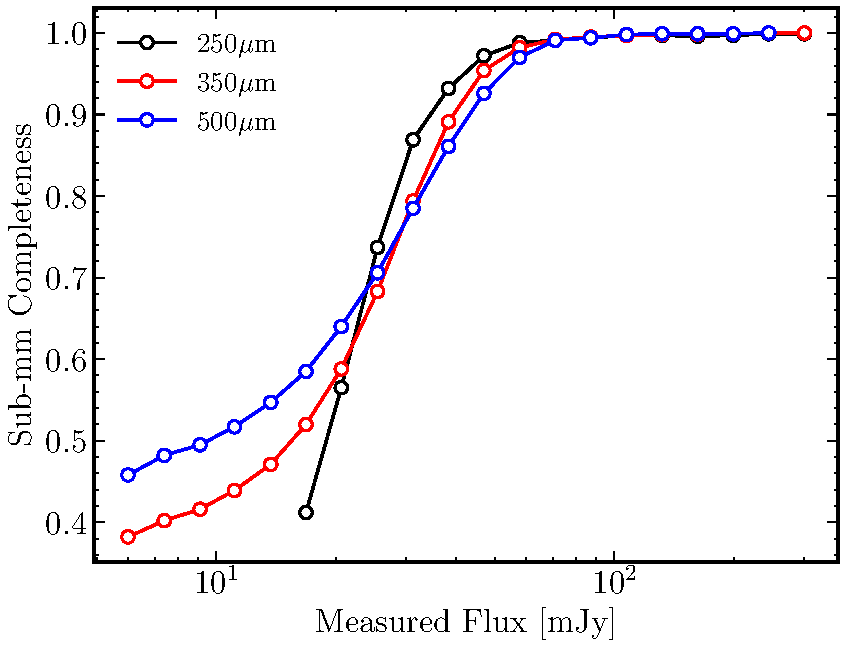
\includegraphics[width=\columnwidth]{Figures/submm_completeness.pdf}
	\caption{The completeness of the H-ATLAS Data Release I catalogues of sub-mm sources, as a function of the measured flux density at 250\,\micron (black) 350\,\micron (red) and 500\,\micron (blue). This figure is replotted from Figure 21 in \citealt{Valiante_2016}.}
	\label{fig:submm_completeness}
\end{figure}

\subsection{Data Releases of the H-ATLAS}
\label{sec:Data Releases of the H-ATLAS}

The first public data release (DR1) of H-ATLAS covered the three equatorial GAMA fields, which span approximately 25\% of the total survey area. These fields benefit from multiwavelength coverage from GAMA, SDSS, 2dF, the Galaxy Evolution Explorer (GALEX, \citealt{Martin_2005}), the UKIRT Infrared Deep Sky Survey -- Large Area Survey (UKIDSS-LAS, \citealt{Lawrence_2007}), the Wide-field Infrared Survery Explorer (WISE, \citealt{Wright_2010}), the VISTA Kilo-degree Infrared Galaxy survey (VIKING, \citealt{Edge_2013}) and the Kilo-Degree Survey (KiDS, \citealt{deJong_2013}). 

Sources are provided with DR1 if they are detected above the 2.5$\sigma$ detection limit on the 250\,\micron map and have measured flux densities greater than the 4$\sigma$ flux density limits in one of the three SPIRE bands (29.6\,mJy, 37.6\,mJy or 40.8mJy at 250, 350 and 500\,\micron). Across the three fields there are a total of 113,995, 46,209 and 11,011 sources detected at > 4$\sigma$ at 250, 350 and 500\,\micron as well as detections for 4,650 and 5,685 sources at > 3$\sigma$ at 100 and 160\,\micron (\citealt{Valiante_2016}). Following the release of the sub-mm sources detected in the GAMA fields, \citealt{Bourne_2016} used the Likelihood Ratio (LR, \citealt{Sutherland_1992}; \citealt{Ciliegi_2003}) method (Section \ref{sec:The Likelihood Ratio Method}) to identify potential optical counterparts to the 113,995 sources with SNR$_{250}$ > 4 from SDSS. Sources with SNR$_{250}$ < 4 that were detected by their 350 or 500\,\micron flux densities were omitted from the matching since these sources have sub-mm colours suggesting a high redshift, and are the most likely sources to be misidentified by SDSS due to the increased probability of chance alignments or gravitational lensing along the line of sight (\citealt{Negrello_2010}; \citealt{Pearson_2013}; \citealt{Bourne_2014}). \citealt{Bourne_2016} found optical counterparts within 10" of 44,385 (39\%) sources with an estimated probability of being the true ID > 80\% (the probability of an optical or near-infrared object being the true counterpart to a sub-mm source is defined as the reliability, R, and is derived in Section \ref{sec:The Likelihood Ratio Method}).

The second public data release (DR2) covered the NGP and SGP, two large fields that together form $\sim$\,75\% of the total survey area. The NGP was covered in the optical by the SDSS and in the near-infrared by UKIDSS-LAS. Moreover, a small area of 25.93\,$\deg^2$ within the NGP was also observed by a deeper K-band survey by the H-ATLAS team using UKIRT (limiting magnitude of K < 19.40 compared to K < 18.69 for UKIDSS-LAS). The SGP is the largest field (approximately half the survey area of H-ATLAS) and was covered by the 2dF spectroscopic survey, KiDS in four optical bands ($u$, $g$, $r$ and $i$) and VIKING in five near-infrared bands ($Z$, $Y$, $J$, $H$ and $K_s$).

Given that sub-mm sources are only extracted from areas of the \textit{Herschel} maps that have at least two obsersations from the SPIRE instrument, the DR2 catalogues includes sources from the map area reduced by the masking of single \textit{Herschel} scans. The mask reduces the area covered by the NGP point source catalogue to 177.1\,$\deg^2$ and the SGP to 303.4\,$\deg^2$. As with DR1, sources are included if they are detected on the 250\,\micron map above the 2.5$\sigma$ detection limit by the MADX algorithm and surpass at least one of the 4$\sigma$ flux density limits at the SPIRE wavelengths. The catalogues contain 118,980 sources for the NGP field (112,069, 48,876 and 10,368 detected at > 4$\sigma$ at 250, 350 and 500\,\micron and 5,036 and 7,046 at > 3$\sigma$ at 100 and 160\,\micron respectively) and 193,527 sources for the SGP field (182,282, 74,096 and 16,084 at 250, 350 and 500\,\micron and 8,598 and 11,894 at 100 and 160\,\micron). \citealt{Furlanetto_2018} applied the Likelihood Ratio method to all counterparts within 10" of the 250\,\micron sources of the NGP using both the shallower optical and near-infrared catalogue of SDSS and UKIDSS-LAS, and the deeper K-band survey. Of the 112,155 SPIRE sources with SNR$_{250}$ > 4, 77,521 (69.1\%) had at least one shallow optical counterpart and 42,429 (37.8\%) of these were matched with R > 0.8. In the smaller area observed with WFCAM, \citealt{Furlanetto_2018} identified 32,041 possible deep near-IR counterparts to 17,247 sources. 10,668 (61.9\%) of these sources were matched with an equally high reliability. While this analysis suggests that the inclusion of deeper K-band data drastically increases the fraction of sources matched to their corresponding optical or near-IR counterpart, [...]\todo[color=yellow]{continuation: we must consider their differences and think about Q}.

In the SGP a preliminary counterpart analysis was conducted using the Two Micron All Sky Survey (2MASS, \citealt{Skrutskie_2006}), but no formal LR analysis had yet been applied. A nearest neighbour match within 5" of a 2MASS galaxy gives identifications for 3,444 \textit{Herschel} sources. In the following section we detail the Likelihood Ratio method and apply it to the 250\,\micron sources detected by \textit{Herschel} in the SGP.

\subsection{Identifying Optical and Near-IR Counterparts to Herschel Sources}
\label{sec:Identifying Optical and Near-IR Counterparts to Herschel Sources}

When identifying multiwavelength counterparts across surveys the simplest choice to use the nearest neighbour within a fixed search radius of one of the sources. For surveys conducted at similar wavelengths with a similar resolution and sensitivity this is a suitable approach. However, when matching far-IR/sub-mm surveys to optical/IR data, the poor angular resolution of long wavelength instruments such as SPIRE (the FWHM of 250\,\micron detections with SPIRE is $\sim$ 18"), which cause large positional uncertainties, force us to increase the search radius around the sub-mm source. This effect, coupled with the intrinsic faintness of optical/near-IR counterparts due to dust obscuration, the relatively flat redshift distribution of sub-mm sources due to the k-correction and the high surface density of objects in optical/IR surveys, means that [...]\todo[color=yellow]{continuation: identification is not easy, Casey reference?} and it is common for there to be multiple possible counterparts within the search radius from a single sub-mm source.

Previously for sub-mm surveys it would be more practical to first match sources with radio or mid-IR sources and then use pre-existing matched catalogues to obtain multiwavelength data (e.g. \citealt{Ivison_2007}; \citealt{Dye_2009}; \citealt{Biggs_2011}, see also Section [...]\todo[color=green]{add reference for the final chapter}). However, presently this is not suitable for large surveys such as H-ATLAS as current radio telescopes do not provide the area and depth required to match with more than a small fraction of sub-mm sources. While current and future radio surveys from facilities such as the Square Kilometre Array (SKA), the Low Frequency Array (LOFAR) and MeerKAT will increase the radio coverage of the H-ATLAS fields, currently a statitstical identification method is still the preferred way of deciding which objects are associated and which are unrelated foreground/background objects to large samples of sub-mm sources.

\subsection{The Likelihood Ratio Method}
\label{sec:The Likelihood Ratio Method}

The Likelihood Ratio method assigns a probability (reliability) to all potential matches surrounding low resolution sources to distinguish between likely counterparts and chance alignments and has been used many times to identify counterparts to \textit{Herschel} sources. The LR method was used by \citealt{Smith_2011} to identify SDSS counterparts in the Science Demonstration Phase (SDP) catalogue (a preliminary data release for H-ATLAS, overlapping with the GAMA9 field), by \citealt{Kim_2012} to identify Spitzer-IRAC counterparts also in the SDP data, by \citealt{Fleuren_2012} for VIKING IDs in the Phase 1 catalogue of the GAMA9 field, and as mentioned earlier, by \citealt{Bourne_2016} and \citealt{Furlanetto_2018} to find optical and near-IR counterparts in the GAMA fields and NGP field respectively.

The likelihood, $L$, of a counterpart being the true identification to a \textit{Herschel} source is given by the ratio between the probability that an object observed at a given radius from the source, $r$, with an optical or near-IR magnitude, $m$, is the true identifcation and the probability of observing an unassociated object with the same $r$ and $m$. On the assumption that the distance from the source and the optical/near-IR magnitude are independent on their influence on the probability of being a true counterpart, we find that:

\begin{equation}
\label{eq:likelihood_ratio}
    L = \frac{P(\textrm{ID}, r, m)}{P(\textrm{unassociated}, r, m)} = \frac{P(\textrm{ID}, r) P(\textrm{ID}, m)}{P(\textrm{unassociated}, r, m)}
\end{equation}

Each term in the above equation can be defined in the following way: $f(r) \coloneqq P(\textrm{ID}, r)$, $q(m) \coloneqq P(\textrm{ID}, m)$ and $n(m) \coloneqq P(\textrm{unassociated}, r, m)$, where $f(r)$ represent the radial probability distribution function of positional errors between the source and counterpart, $q(m)$ represents the magnitude probability distribution of true counterparts and $n(m)$ is the magnitude distribution of background objects from the input survey. By using Baye's theorem and the theorem of total probability, we can define the probability that a counterpart is the true ID given it has $r$ and $m$ as:

\begin{equation}
\label{eq:reliability_one_counterpart}
    R \coloneqq P(\textrm{ID}| r, m) = \frac{L}{L+1}.
\end{equation}
\todo[color=green]{Requires a derivation}

Equation \ref{eq:reliability_one_counterpart} assumes that there is only a single candidate with a likelihood $L$. For a source with multiple possible candidates, the reliability $R_j$ of the $j^{th}$ candidate is given by:

\begin{equation}
    \label{eq:reliability_multiple_counterparts}
        R_j = \frac{L_j}{\sum_i L_i + (1-Q)},
\end{equation}

where $i$ represents the $i^{th}$ counterpart found within the search radius. The $Q$ parameter represents the fraction of all true counterparts that are brighter than the limiting magnitude of the input survey and can therefore be observed. This means that the (1 - $Q$) term represents the probability that the counterpart is not observed and accounts for the fact that not all counterparts will be detected in the optical/near-IR survey. The value of $Q$ depends on the depth of the survey and the choice of passband used. In the following sections I shall outline the methods used to estimate the functions $f(r)$, $q(m)$ and $n(m)$ and to estimate $Q$ to calculate the likelihood ratios and reliabilities of near-IR counterparts observed on the VIKING images surrounding the 250\,\micron positions of \textit{Herschel} sources in the SGP.

\section{Applying the LR Method to VIKING Galaxies in the SGP}
\subsection{VISTA VIKING Counterparts}

The Visible and Infrared Survey Telescope for Astronomy (VISTA) is a 4\,m wide field telescope located at the ESO Paranal Observatory in Chile. The telescope has five near-IR broad band filters, $Z$, $Y$, $J$, $H$ and $K_s$, that have central wavelengths between 0.88 and 2.15\,\micron (\citealt{Emerson_2010}). The VIKING survey was a public survey with VISTA, covering approximately 1,500\,$\deg^{2}$ of sky, including an overlap of more than 360\,$\deg^{2}$ with the H-ATLAS survey in the GAMA and SGP fields, to a 5\,$\sigma$ depth of 23.1, 22.3, 22.1, 21.5 and 21.2 (AB) in the above five filters.

We take as our object catalogue all objects observed in the fourth data release of VIKING within 15" of the 250\,\micron position of each \textit{Herschel} source. The counterpart matching in the GAMA9 field by \citealt{Fleuren_2012}, recovered 51\% of all 250\,\micron sources with a reliable (R > 0.8) VIKING counterpart. Compared to the optical r-band of the SDSS as used in \citealt{Bourne_2016} and \citealt{Furlanetto_2018} which have typical returns of $\sim$ 35 -- 40\% due to the limiting magnitude of SDSS, we expect the SGP to have reliable identifications for approximately half of all SGP sources. The SGP fields contains 193,527 sources detected at greater than 4\,$\sigma$ significance, suggesting that we might expect to match $\sim$ 100,000 \textit{Herschel} sources with a near-IR counterpart with a high probability.

However, a significant number of sources in the VIKING survey are stars that would be erroneously matched to H-ATLAS. The sub-mm emission from stars is most likely from debris discs or dust in outflows. As there is large variation in the mass and temperature of debris discs for stars of a given spectral type (\citealt{Hillenbrand_2008}), and \textit{Herschel} is only sensitive to the brightest of these discs (\citealt{Thompson_2010}), there is much scatter in the sub-mm properties of \textit{Herschel} detected stars which would result in poor statistics of dusty stars when calculating the likelihood of counterparts. For this reason, I use an adapted method of \citealt{Baldry_2010} to separate stars and galaxies in the VIKING SGP catalogue and apply the LR method separately for the two classes.

The method of \citealt{Baldry_2010} uses near-IR $J$ and $K_s$ and optical $g$ and $i$ bands to define a line of separation between stars and galaxies in $J - K_s$, $g-i$ colour-colour space, and is used in \citealt{Bourne_2016} and \citealt{Furlanetto_2018} to separate stellar and extragalactic objects in SDSS. Without coverage from SDSS in the SGP, I use the fourth data release of KiDS to identify optical $g$ and $i$ bands for [...]\todo[color=green]{Look up value} of our VIKING sources. A nearest neighbour search to a maximimum of 0.5" from the 250\,\micron position of each source was used.

First, I classify as stellar any object in our catalogue with \texttt{pStar} > 0.95, an estimate of the probability that the source is a star, based on a shape parameter provided as part of the VIKING data release. This immediately classifies 51,508 objects as stars. Next I consider the $J - K_s$, $g-i$ colour-colour space and define a stellar locus by converting the locus in \citealt{Baldry_2010} to the Vega system assuming $J_{\textrm{Vega}}$ = $J_{\textrm{AB}}$ - 0.91 and $K_{s,\textrm{Vega}}$ = $K_{s,\textrm{AB}}$ - 1.85:

\begin{equation}
    f_{\textrm{locus}} = 
    \begin{cases*}
        0.228 & $g-i$ < 0.3 \\
        0.05 + 0.615(g-i) - 0.13(g-i)^2 & 0.3 $\leq$ $g-i$ < 2.3 \\
        0.7768 & $g-i$ $\geq$ 2.3.
    \end{cases*}
\label{eq:stellar_locus}
\end{equation}

I define a line of separation between stars and galaxies as being +0.2 offset in $J - K_s$ from the stellar locus. The distribution of sources, stellar locus and separation line are illustrated in Figure \ref{fig:star_galaxy_classification}. This classifies a further 411,463 sources that have KiDS identifications (299,525 extragalactic and 111,938 stellar). The remaining objects do not have matches in KiDS and thus do not have $g$ and $i$-band magnitudes. However, based on the separation line defined above, it can be seen that those objects with $J - K_s$ < 0.42 will always fall below the separation line regardless of their optical colour, and similarly, any object with  $J - K_s$ > 0.98 will always lie above the line. The cross contamination of stars above the line and galaxies below the line is small, so I next define all remaining sources using the above single flux cuts. This classifies a further 102,540 sources (102,265 as galaxies and 275 as stars). Finally, I return to the \texttt{pStar} parameter and relax the criteria to those objects with \texttt{pStar} > 0.7; all other objects are classified as galaxies. This method leads to the identifcation of 793,331 (78.9\%) extragalactic sources and 212,028 (21.1\%) stars.

\begin{figure}
	\includegraphics[width=\columnwidth]{Figures/star_galaxy_classification.pdf}
	\caption{The $J - K_s$, $g-i$ colour-colour diagram of VIKING objects with KiDS identifications in the SGP. The stellar locus defined by Equation \ref{eq:stellar_locus} is illustrated as the blue line, while the separation between stars and galaxies, defined as +0.2 offset from the stellar locus, is shown as a dashed blue line. Extragalactic and stellar sources identified from our classification are shown as grey and red points respectively.}
	\label{fig:star_galaxy_classification}
\end{figure}

\subsection{Distribution of True Counterparts, q(m)}
\label{sec:true_counterparts_distribution}

To estimate the reliability of each VIKING source being the true ID to a \textit{Herschel} source, I determine the probability distribution of true counterparts as a function of $K_s$-band magnitude, $q(m)$, using the method described in \citealt{Ciliegi_2003}. First, a magnitude distribution of all objects found in the VIKING images within 15" of a \textit{Herschel} source is generated separately for stars and galaxies, which we shall denote as $n'_{\textrm{total}}(m)$. Here I have set prime notation to reference raw counts, while no prime notation is reserved for counts that have been normalized by the total area searched on the VIKING images. The excess of sources above the background level in regions surrounding the 250\,\micron sources is an estimate for the number density of true VIKING associations and is estimated by subtracting the magnitude distribution for the whole VIKING survey from $n'_{\textrm{total}}(m)$. A set of 844,715 random positions were located on the SGP map and used to search for objects on the VIKING images to within 15". A total of 2,917,214 objects were found and form our $n'_{\textrm{background}}(m)$ distribution. The excess of "real" counterparts thus has a magnitude distribution that may be expected to follow

\begin{equation}
    n'_{\textrm{real}}(m) = n'_{\textrm{total}}(m) - n'_{\textrm{background}}(m) \frac{N_{\textrm{250\,\micron}}}{N_{\textrm{background}}},
\end{equation}

where the distribution has been scaled to the search area by $N_{\textrm{250\,\micron}}$ and $N_{\textrm{background}}$, the number of 250\,\micron positions and the number of randomly located positions respectively.

I then derive the $q(m)$ distribution by normalizing $n_{\textrm{real}}(m)$ and scaling by the fraction of all true counterparts that would be visible on the VIKING images, $Q$. This ensures that the integral of $q(m)$ over all magnitudes up to the limiting magnitude of the VIKING survey is equal to the probability that the sources is detected, i.e. $\int^{m_{\textrm{lim}}} q(m)dm = Q$. This normalization can be written as:

\begin{equation}
\label{eq:true_counterparts_distribution}
    q(m) = \frac{n'_{\textrm{real}}(m)}{\sum_{m_i}n'_{\textrm{real}}(m_i)}\times Q,
\end{equation}

where we have summed over the magnitude bins, $m_i$. The magnitude distribution of "true" counterparts to the 250\,\micron SGP sources is illustrated in the middle panel of Figure \ref{fig:true_counterparts_distribution} and shows the difference between the two distributions for extragalactic and stellar sources, requiring us to implement the LR method separately for the two classes. I also show in Figure \ref{fig:true_counterparts_distribution} the magnitude distributions of $n_{\textrm{total}}$ and $n_{\textrm{background}}$ and the distributions $q(m)/n(m)$ (here $n(m)$ references the area-normalized background distribution of sources, as used in Equation \ref{eq:likelihood_ratio} to calculate the likelihood values). The calculation of the likelihood value for each VIKING source thus depends on an estimate for the fraction of true IDs that are observed on the VIKING images, $Q$, which I detail in the following section.

\begin{figure}
    \centering
	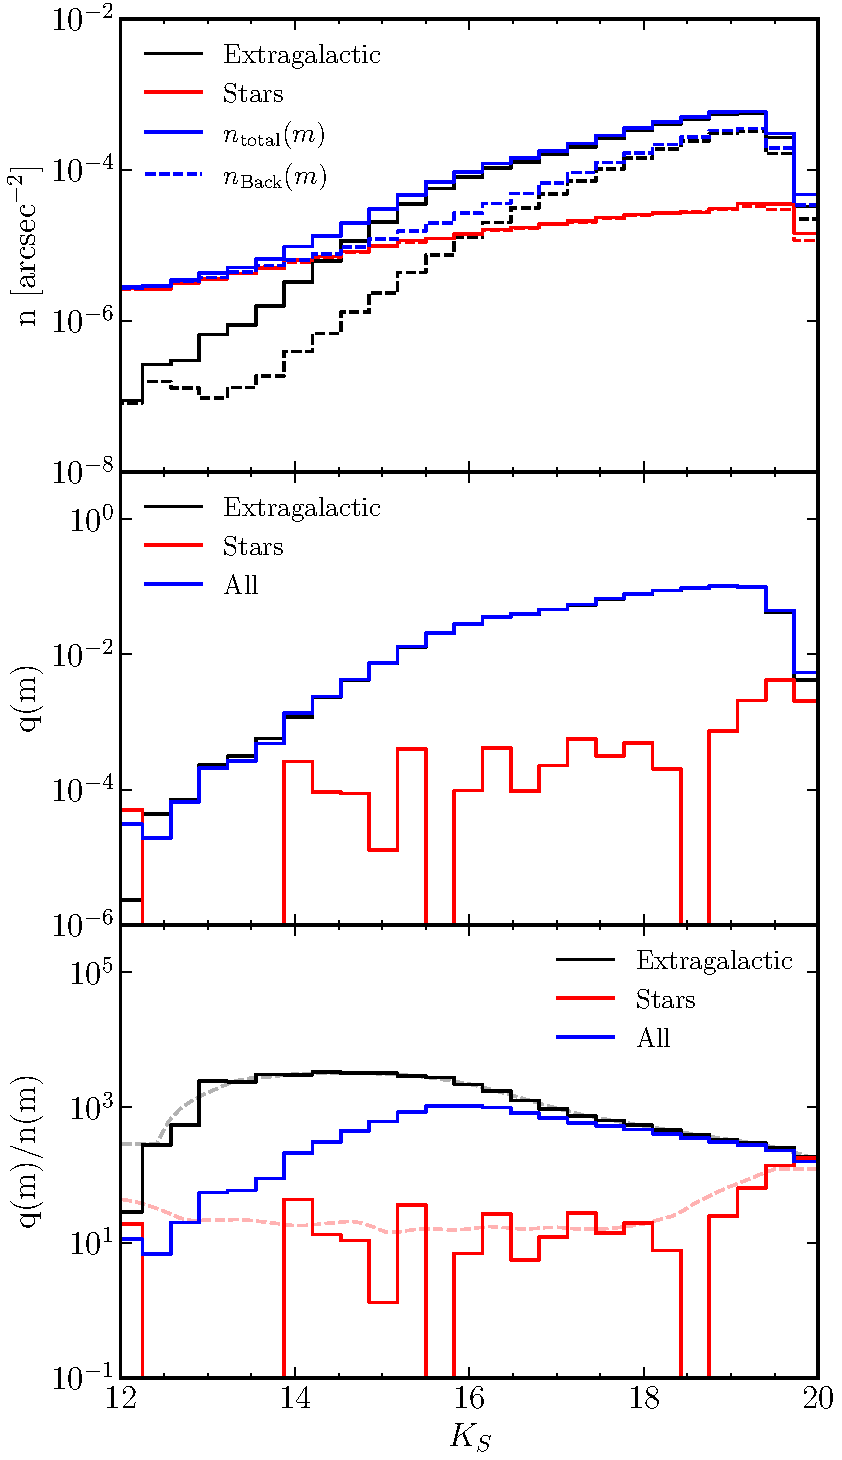
\includegraphics[height=0.75\textheight]{Figures/true_counterparts_distribution.pdf}
	\caption{Top panel: The $K_s$-band magnitude distributions of objects located within 15" of 250\,\micron \textit{Herschel} positions (blue solid line) and random positions (blue dashed line), also separated by extragalactic (black lines) and stellar (red lines) identifications. Middle panel: The $K_s$-band magnitude distribution of "true" counterparts accounting for the excess of VIKING sources observed near \textit{Herschel} sources. Bottom panel: The ratio between the "true" counterparts distribution (middle panel) and the background distribution of sources, as used in the calculation of likelihoods; Equation \ref{eq:likelihood_ratio}. The dashed lines represent smoothed fits to $q(m)/n(m)$ to provide a continuous function at all magnitudes. The colour convention of the middle and bottom panels are the same as the top panel.}
	\label{fig:true_counterparts_distribution}
\end{figure}

\subsection{Estimating Q}

I predict the probability of finding a genuine counterpart in the VIKING images above the limiting magnitude using the method described in \citealt{Fleuren_2012}. While some methods estimate $Q$ directly by totaling the $n_{\textrm{real}}(m)$ distribution and dividing by the number of SPIRE sources, this leads to a systematic overestimate due to the possibility of clustering of galaxies or multiple counterparts to the sub-mm source due to source blending. An alternative method by \citealt{Fleuren_2012} calculates an estimate of 1-$Q_0$, the probability of not observing a VIKING counterpart, by counting the number of sub-mm sources without VIKING associations within a search radius, $r$. These sources will be given the name \textit{blanks}, and has a dependency on search radius, $B(r)$.

Blank sources may be observed in one of several scenarios. The most likely reason (given the limiting depth of VIKING compared to \textit{Herschel}, see Figure [...]\todo[color=orange]{If I include a plot that compares the depth of the surveys against Herschel limits, add reference here.}) is that the real source is fainter than the VIKING $K_s$-band limit. However, a blank may also be observed if the counterpart lies outside the search radius or if the sub-mm source is a spurious SPIRE detection.

While we may observe a sub-mm source with a possible VIKING candidate, we may not definitively say that a source is not a blank as we may encounter chance alignments with VIKING sources close to the same line of sight. Thus, to estimate the true number of blanks, we are reminded that the number of blanks we observe must also account for those that are spuriously identified as not blank. In other words, the number of observed blanks is the number of true blanks minus the number of true blanks that have random VIKING interlopers. If we define the number of observed blanks as $B_{\textrm{obs}}$, the number of true blanks as $B_{\textrm{t}}$ and the number of random interlopers as $N_{\textrm{rand}}$, then

\begin{equation}
    B_{\textrm{obs}} = B_{\textrm{t}} - N_{\textrm{rand}} = B_{\textrm{t}} - B_{\textrm{t}} \times f_{\textrm{rand}},
\end{equation}

where we have assumed that the number of random interlopers can be estimated from the fraction of positions that have random interlopers, $f_{\textrm{rand}}$. This fraction can be estimated from the set of random positions used above to calculate $q(m)$. Using a similar set of notation: $B_{\textrm{background}}$ to represent the number of blank positions from the catalogue of random positions; $N_{\textrm{background}}$ to represent the number of random positions; and $B'_{\textrm{background}}$ representing the number of random positions for which a VIKING counterpart was observed (or non-blank), we can estimate $f_{\textrm{rand}}$ as:

\begin{equation}
    f_{\textrm{rand}} = \frac{B'_{\textrm{background}}}{N_{\textrm{background}}} = \frac{N_{\textrm{background}} - B_{\textrm{background}}}{N_{\textrm{background}}} = 1 - \frac{B_{\textrm{background}}}{N_{\textrm{background}}}.
\end{equation}

To scale this fraction to the size of the SPIRE catalogue, the same number of random positions are used as there are 250\,\micron positions, such that $f_{\textrm{rand}}$ may be written as:

\begin{equation}
    f_{\textrm{rand}} = 1 - \frac{B_{\textrm{background}}}{N_{\textrm{250\,\micron}}}.
\end{equation}

From substitution we find that the fraction of \textit{Herschel} sources that are true blanks (i.e. $B_{\textrm{t}}/N_{\textrm{250\,\micron}}$), is given by:

\begin{equation}
    \frac{B_{\textrm{t}}}{N_{\textrm{250\,\micron}}} = \frac{B_{\textrm{obs}}}{B_{\textrm{background}}}.
\end{equation}

In summary, to estimate 1-$Q$, we need only to divide the number of observed blank 250\,\micron positions by the number of observed blank random positions. It is clear that any estimate of $Q$ using this method depends on the given search radius from the sub-mm source, $r$, thus I calculate this fraction for a range of radii between 0" and 15" and model the dependence of $B(r) \coloneqq 1 - Q$ on the search radius in the same manner as \citealt{Fleuren_2012}. 

A sub-mm source that has no true VIKING association within a radius $r$ is either a source whose counterpart is too faint to be detected by the VIKING survey or lies outside the radius, or both. Assuming that such situations are independent of each other (i.e. a true VIKING candidate that lies at higher offsets from the sub-mm source than average is not also fainter and vice versa), then the probability of either occurring is given by the conditional probability:

\begin{equation}
    P(\textrm{Blank}) = P(\textrm{Faint} \cup \textrm{Outside}) = P(\textrm{Faint}) + P(\textrm{Outside}) - P(\textrm{Faint} \cap \textrm{Outside}).
\end{equation}

The first term, the probability that the counterpart is too faint to be detected is given by 1-$Q$, while the probability that the counterpart resides outside the search radius is dependent on the distribution of offsets between the counterpart and sub-mm source, $f(r)$. This distribution represents the probability that a real counterpart is found at a radial distance $r$ from the SPIRE source, where we assume that the H-ATLAS sources are point-like on the 250\,\micron maps and that the errors are equal in RA and declination for radial symmetry.

While $f(r)$ depends on both the positional errors of the sub-mm and the VIKING catalogues, we can assume that the near-IR positional errors are negligible compared to those of SPIRE given that the 1$\sigma$ VIKING positional errors are < 0.2" (\citealt{Fleuren_2012}), while the FWHM of the 250\,\micron beam used to extract the \textit{Herschel} sources is $\sim$ 18". As such, I use a radially symmetric Gaussian with width $\sigma_\textrm{pos}$ as $f(r)$. Accordingly with the theory of total probability, the probability that an observable counterpart is detected out to any search radius must equal unity, thus our function $f(r)$ is normalized such that:

\begin{equation}
    \int_0^\infty 2\pi f(r')r'dr' = 1,
\end{equation}

which implies for our Gaussian distribution that

\begin{equation}
    f(r) = \frac{1}{2\pi\sigma_\textrm{pos}^2}e^{\frac{-r^2}{2\sigma_\textrm{pos}^2}}.
\label{eq:positional_offset_distribution}
\end{equation}
[...]\todo[color=orange]{Requires a derivation.}

Returning to the probability that a VIKING counterpart is not observed within a radius $r$, we can estimate this as 1 - $F(r)$ where $F(r)$ relates to $f(r)$ as

\begin{equation}
    F(r) = \int_0^r 2\pi r'f(r')dr'.
\end{equation}

Upon substitution we thus find that the probability of observing a blank source as a function of the search radius can be modelled as

\begin{equation}
    B(r) = P(\textrm{Blank}) = (1-Q) + (1-F(r)) - (1-Q)(1-F(r)) = 1 - QF(r)
\label{eq:blanks_model}
\end{equation}

In Figure \ref{fig:Q_estimate} I show the observed number of blank \textit{Herschel} (open squares) and random (open circles) positions as a function of the search radius, as well as their ratio which is our estimate of $B_{\textrm{t}}/N_{\textrm{250\,\micron}}$ (filled circles). The best fitting $B(r)$ is illustrated as the black line. Using this method I estimate the value of $Q$ to be $0.835\pm0.009$ when considering all VIKING objects and $Q=0.823\pm0.009$ when stellar contaminants are removed.

\begin{figure}
    \centering
	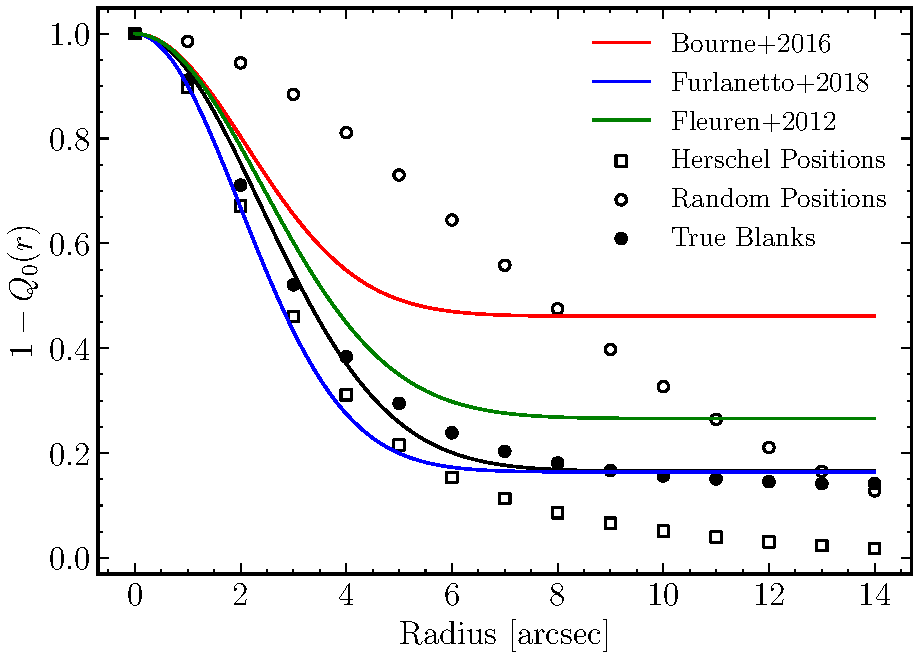
\includegraphics[width=\columnwidth]{Figures/Q_estimate.pdf}
	\caption{Estimates for the number of blanks (sources without VIKING candidates) as a function of the search radius, $r$. Open circles represent the number of blank random positions placed across the SGP, while open squares represent the number of blank SPIRE 250\,\micron positions from H-ATLAS. The filled circles shows the division of the former by the latter, representing our estimate for the true fraction of SPIRE sources that are blank on the VIKING images. The solid black line represents the best fit to the points using Equation \ref{eq:blanks_model}. The same model used in \citealt{Fleuren_2012}, \citealt{Bourne_2016} and \citealt{Furlanetto_2018} are shown as green, red and blue lines respectively.}
	\label{fig:Q_estimate}
\end{figure}

Previous estimates of $Q$ from r-band SDSS candidates in the other H-ATLAS fields have taken lower values as a result of the difference in depth between SDSS and VIKING. In DR1 \citealt{Bourne_2016} measured the value of $Q$ for all SDSS objects observed in the GAMA fields to be $0.539\pm0.001$, and \citealt{Furlanetto_2018} measured a near identical value of $Q=0.538\pm0.001$ in the NGP during DR2. However, my value of $Q$ is similar to that found by \citealt{Fleuren_2012}, $Q = 0.7342\pm0.0257$ and is almost identical to the value of $0.836\pm0.001$ found from the deep K-band analysis by \citealt{Furlanetto_2018}. As a collection, these estimates indicate that a survey of VIKING candidates returns a greater probability of observing a galaxy near a sub-mm source than an SDSS survey due to the increase in depth. A comparison between data releases due to the available input survey is made in Section [...]\todo[color=orange]{If a comparison between data releases is made, add the section reference here.} and in Table \ref{tab:data_release_input_surveys} I detail the various estimates made for $Q$ during analyses of H-ATLAS sources alongside their input surveys, passbands used and their depths.

\begin{table}
\centering
\begin{tabular}{|p{6.5cm}|p{3.5cm}|p{2.5cm}|p{4cm}|}
    \hline
    H-ATLAS & Input Survey & $Q$ Estimate & Reference \\
    \hline
    \hline
    Science Demonstration Phase (SDP) & SDSS -- ($r < 22.4$) & $0.583$ & \citealt{Smith_2011} \\ 
    Phase 1 GAMA9 & VIKING -- ($K_s < ??$) & $0.734\pm0.026$ & \citealt{Fleuren_2012} \\
    Data Release I & SDSS -- ($r < ??$) & $0.539\pm0.001$ & \citealt{Bourne_2016} \\
    Data Release II & SDSS -- ($r < ??$) & $0.538\pm0.001$ & \citealt{Furlanetto_2018} \\
    Data Release II & UKIRT -- ($K_s < ??$) & $0.836\pm0.001$ & \citealt{Furlanetto_2018} \\
    Data Release III & VIKING -- ($K_s < ??$) & $0.835\pm0.009$ & This work \\
    \hline
\end{tabular}
\caption{Comparison of the input survey passbands, depths and measured values of $Q$. From left to right the columns contain: i) the corresponding data release of H-ATLAS, ii) the input survey, passband used and its limiting magnitude, iii) the fraction of true sources observed on the survey images, $Q$, iv) reference.}
\label{tab:data_release_input_surveys}
\end{table}
\todo[color=orange]{Complete Table.}

\subsection{Positional Uncertainty of H-ATLAS Detections}

The fitting function of Equation \ref{eq:blanks_model} also provides an estimate for the standard positional error, $\sigma_{\textrm{pos}}$ which defines the width of the positional offset distribution $f(r)$. I measure this value to be $\sigma_{\textrm{pos}} = 2.388\pm0.065"$, representing the average error in the 250\,\micron positions. We see in Figure \ref{fig:Q_estimate} that $B(r)$ becomes flat at approximately 3$\sigma_{\textrm{pos}}$, suggesting that few counterparts are to be found at search radii greater than $\sim$ 7". It also interesting to note that the model underpredicts the number of blank sources between 4 $\lesssim$ r $\lesssim$ 8 arcsec, but overpredicts at the highest search radii. This has been observed previously (e.g. \citealt{Fleuren_2012}) and might suggest clustering of VIKING objects which is not modelled in $B(r)$.

The positional uncertainty has a dependency on the SNR of the sub-mm detection (\citealt{Bourne_2016}) and in theory should depend on the ratio between the FWHM of the observations and the SNR as given by

\begin{equation}
    \sigma_{\textrm{pos}} = 0.6\times\frac{\textrm{FWHM}}{\textrm{SNR}},
\label{eq:positional_uncertainty_theory}
\end{equation}

as detailed by \citealt{Ivison_2007} on the assumption of uncorrelated noise. However, the prefactor is likely to be increased by confusion noise in the maps and clustering (\citealt{Chapin_2011}; \citealt{Bourne_2014}) and so a scaling factor (typically about 1.09, corresponding to a redefined prefactor of $\sim$ 0.65) is applied and is more suitable for sources detected on sub-mm images. To define an individual value of the 1$\sigma$ positional uncertainty, and thus a separate $f(r)$ for each detection, I implement an empirical version of Equation \ref{eq:positional_uncertainty_theory} of the form

\begin{equation}
    \sigma_{\textrm{pos}} = k\times\frac{\textrm{FWHM}}{\textrm{SNR}},
\label{eq:positional_unceratinty_empirical}
\end{equation}

where $k$ is a constant to be determined. Using FWHM = 18", the fitted value of $\sigma_{\textrm{pos}} = 2.388$ and  the SNR of each 250\,\micron detection, I generate a set of $k$ values. I take the median value of the distribution of $k = 0.66$ as my constant. This value is used in Equation \ref{eq:positional_unceratinty_empirical} to determine $f(r)$ for each object's likelihood calculation.

A more refined method of determining $\sigma_{\textrm{pos}}$ is outlined in \citealt{Smith_2011} and applied in other works (e.g. \citealt{Bourne_2014}, \citealt{Bourne_2016} and \citealt{Furlanetto_2018}), though is also an empirical measurement. In such studies, a 2D histogram is derived for the offsets between sub-mm sources and optical/near-IR objects within a large box around each SPIRE source (typically 50" or more). This histogram can be modelled in shape by three contributing populations: i) a random background of chance alignments which should be observed as a constant since the probability of a chance alignment is equal along any line of sight; ii) the population of true IDs whose positional offset distribution follows $f(r)$ for a fraction $Q$ of all sources and iii) nearby counterparts that are physically correlated with the sub-mm source due to galaxy clustering but are not the true IDs, which requires an understanding of the cross-correlation between the sub-mm and optical/near-IR samples. Further details on the modelling of these histograms can be found in \citealt{Smith_2011}. By binning the sub-mm sources by their SNR and fitting the 2D histograms with a model considering the above contributions, an estimate can be made for $\sigma_{\textrm{pos}}$ as a function of SNR. Assuming a powerlaw dependence of the form $\sigma_{\textrm{pos}} = \sigma_{\textrm{pos}}(5) [\textrm{SNR}/5]^\alpha$ where $\sigma_{\textrm{pos}}(5)$ is the positional uncertainty of a 250\,\micron detection with SNR = 5, and by binning the sources further by sub-mm colour, it has been shown that the bluest SPIRE sources ($S_{250}/S_{350}$ > 2.4) have a dependence of $\sigma_{\textrm{pos}}$ on SNR that is not significantly different from the theoretical model given in Equation \ref{eq:positional_uncertainty_theory} (\citealt{Bourne_2016}; \citealt{Furlanetto_2018}). As shown in these studies the powerlaw function shifts to higher values of $\sigma_{\textrm{pos}}$ as we tend to redder sources. A possible explanation for a broader distribution of offsets for redder SPIRE sources is due to an increased probability of these sources being at higher redshifts and thus an increased contribution of foreground structures lensing the source. To avoid this bias, $\sigma_{\textrm{pos}}$ could be measured from the 2D histogram of positional offsets of the bluest sources, but for a model dependence that is reasonable for the majority of sources, a multiplicative factor should be included, leading to the prefactor of $k$ commonly assumed being larger than 0.6. Given that the simple method used here provides a similar value of $k$, I do not expect there to be any systematic differences in the likelihood calculations for SGP sources and the aforementioned papers as a result of the different methods used to calculate $\sigma_{\textrm{pos}}$.

\section{Likelihood Ratio Results}

I apply the likelihood ratio to all possible VIKING counterparts within 15" of a SPIRE source. The catalogue contains 193,527 sub-mm sources, of which 190,788 have at least one possible counterpart identified within the search radius. Within this sample, 180,030 are sources with SNR$_{250}$ > 4. Having identified each source with its highest reliability counterpart I find that 181,373 (95.1\%) are sources with VIKING identifications indicating the source is a galaxy and 9,415 (4.9\%) with stellar classifications. 

In keeping with previous studies I define reliable matches as those sources with counterparts having $R \geq 0.8$ in order to minimize the number of false counterparts while maintaining a sample that is dominated by sources with a low chance of blending and thus the FIR emission is likely dominated by a single source. I identified 111,065 reliable near-IR counterparts, representing 58.2\% of all sources with at least one possible candidate. Of the reliable IDs, 110,374 (99.4\%) are classified as extragalactic and 691 (0.6\%) as stellar. The increase in the fraction of galaxies and reduction in stars compared to the input VIKING survey suggests that the LR method is highly biased against stars as is intended.

On the assumption that a source that is erroneously matched with a counterpart has a probability of $1 - R$, we can estimate the false ID rate for our reliable matches:

\begin{equation}
    N_{\textrm{False}} = \sum_{R_i \geq 0.8} (1 - R_i) = 5,343.
\label{eq:false_ids}
\end{equation}

I predict that there are 5,343 "false reliable" IDs in the SGP, representing 4.8\% of the reliable sample. This can be compared to values of 4.7\% in the GAMA fields and the NGP (optical SDSS matching), 4.5\% for the NGP (near-IR deep matching) and 4.2\% during the SDP. While the value for the SGP is in keeping with the other H-ATLAS fields, it is the highest false identification rate. It would be expected that the near-IR analyses would have the lowest false identification rates as the optical r-band restricts the limiting redshift of the counterparts to lower redshifts than the near-IR K-band (see Figure [...]\todo[color=orange]{If a figure showing the different redshift depths of surveys is made, add reference here}). As a result, the contamination of high redshift sub-mm sources that are falsely identified with low redshift optical counterparts is expected to be higher, increasing the false identification rate. However, in the analysis of the SGP, we choose to use an increased search radius of 15" (compared to 10" as used in previous H-ATLAS studies) which increases the average number of counterparts found per source. Given the requirement of the LR method that the sum of the reliabilities of all possible candidates to a source must not exceed one, the increased average number of candidates reduces the average reliability of the true ID and thus increases the false identification rate - likely by a factor greater than the reduction caused by using the near-IR VIKING survey compared to SDSS. Further discussion on the effect of increasing the search radius is made in Section X [...]\todo[color=green]{Add reference to multiplicity section}. The initial choice to use a search radius of 15" came from recent studies suggesting that genuine associations are found on the VIKING images beyond 10" as a result of gravitational lensing (\citealt{Bakx_2020}). In the final SGP \textit{Herschel}+VIKING catalogue, we wish to keep such VIKING objects despite them being highly unlikely to have significant reliability values.

The completeness, $\eta$, of the reliable sample is defined as the fraction of 250\,\micron sources that are recovered with a reliability greater than 0.8 (\citealt{Smith_2011}) and can be estimated as

\begin{equation}
    \eta = \frac{n(R \geq 0.8)}{n(\textrm{SNR}_{250} \geq 4) \times Q},
\label{eq:completeness}
\end{equation}

where the numerator is the size of the reliable sample and the denominator estimates the true number of sources. As would be expected, a value of unity for $\eta$ would imply that the fraction of all counterparts deemed reliable has reached its theoretical maximum, $Q$. Another important diagnostic is the cleanness, $C$, of the reliable ID sample, an estimate for the number of sources that are not spurious matches, given by

\begin{equation}
    C = 1 - \frac{N_{\textrm{False}}}{N_{\textrm{250\,\micron}}}.
\label{eq:cleanness}
\end{equation}

At a reliability cut of 0.8, I find that the completeness of the extragalactic reliable sample is $\eta$ = 78\%, which is similar to the completeness values found for the NGP and GAMA fields of 74\% and 73\% respectively. In Figure \ref{fig:completeness_and_cleanness} I illustrate how the completeness and cleanness change over a range of different reliability thresholds. We see that a cut at $R \geq 0.8$ selects a highly clean sample at the expense of completeness. While an increase in the reliability cut would yield a marginally cleaner sample, it would be offset drastically by a fall in completeness. A decrease in the choice of minimum reliability would lead to an increase in completeness at little expense of the cleanness, but to maximize the completeness would be to set a reliability so low that a one-to-one matching between sub-mm sources and counterparts would not be a guarantee. At $R \geq 0.8$ we set a boundary for which there is a good compromise between the two diagnostic parameters.

\begin{figure}
    \centering
	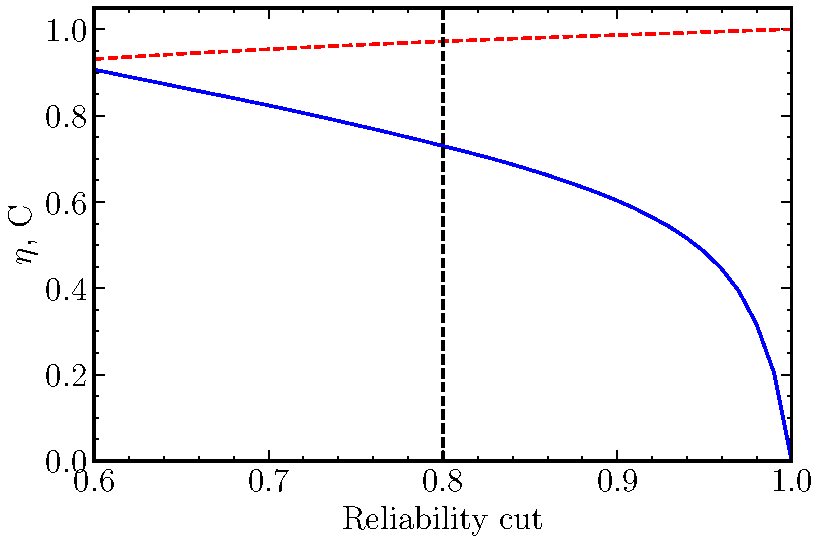
\includegraphics[width=\columnwidth]{Figures/completeness_and_cleanness.pdf}
	\caption{The completeness, $\eta$, and cleanness, C, of the SGP sample as a function of various minimum cuts in reliability, illustrated as solid blue and red dashed lines respectively. The vertical dashed line reprents the reliability cut used in all H-ATLAS fields (R $\geq$ 0.8).}
	\label{fig:completeness_and_cleanness}
\end{figure}

\section{Properties of \textit{Herschel} Sources and their Counterparts}

In the subsequent sections I report on the bulk properties of the SMGs in the SGP field that can be obtained from a combination of the sub-mm and near-IR data. While the far-IR to sub-mm wavebands unveil the dusty, cold regions of the Universe, the inclusion of the near-IR data (the $K_s$-band covers wavelengths between $\sim$ 2--2.3\,\micron) samples the peak of the emission of older stars and as such is suited for examining the stellar properties of a galaxy such as its stellar mass as it traces the total stellar content of a galaxy (\citealt{Cole_2001}; \citealt{Bell_2003}). Moreover, at high redshifts (z $\gtrsim$ 0.5) the rest frame optical bands are observed in the near-IR, meaning that the VIKING counterparts at higher redshifts also probe young stellar populations.

\subsection{Submillimeter Colours}
% Include a comparison of sub-mm colours across the data releases
\subsection{Near-IR Properties of \textit{Herschel} Sources}
% Include a comparison of magnitude distributions

\subsection{Multiplicity of Counterparts}
One important disadvantage to using the LR method to identify multiwavelength counterparts to low resolution sources is that it assumes a one-to-one matching of sources and counterparts. Given that we are restricted to a user defined reliability threshold for our sample, and that the sum of reliabilities for all possible candidates to a source may not exceed one, our reliable sample becomes biased against multiple systems, such as merging galaxies, members of a cluster or non-physical associations such as confusion due to blending, as their combined reliabilities reduces the maximum reliability of the chosen ID. For example, consider two galaxies that form part of a cluster that are observed with VIKING close to a SPIRE source. It is reasonable to imagine that these two sources may have similar K-band magnitude and radial offset from the source, and particularly if they are close to the sub-mm emission, may both have high likelihoods. In such a case, either source may be considered the true ID to the source (and in reality both are likely associated), but the use of Equation \ref{eq:reliability_multiple_counterparts} to define their reliabilities leads to the following simplification (assuming the likelihoods are much larger than $1-Q$):

\begin{equation}
    R_j \sim \frac{L_j}{\sum_i L_i} \sim \frac{L_j}{2L_j} \sim 0.5.
\end{equation}

In this scenario, neither counterpart would be considered the true ID and thus we are biased against multiple systems. 

In Table \ref{tab:multiplicity} I show the number of SPIRE sources and the fraction of those with reliable counterparts as a function of the number of possible candidates observed within 15". We observe that the fraction of sources with reliable counterparts decreases with increasing multiplicity. This suggests that the sample is in part incomplete because we miss sources where there is more than one genuine counterpart. In Figure \ref{fig:multiplicity} I show the reliable fraction of sources as a function of multiplicity for the SGP compared with previous H-ATLAS data releases in other fields. Comparing to the Science Demonstration Phase (\citealt{Fleuren_2012}), GAMA (\citealt{Bourne_2016}) and the NGP (\citealt{Furlanetto_2018}), we see that reliability fraction declines more slowly, peaks at slightly higher average $N_{\textrm{Match}}$ and is lower for sources where there is only a single possible counterpart. These effects are most likely a result of the increased search radius of 15" used during the SGP analysis compared to 10" in the other fields, which per source equates to a 2.5 factor increase in the search area ($A_{\textrm{SGP}}/A_{\textrm{Other}} = \pi r_{\textrm{SGP}}^2/\pi r_{\textrm{Other}}^2 = 225\pi/100\pi = 2.5$). The increased $r$ means that we are more likely to observe a reliable counterpart, but also means we increase the probability of matching erroneously to a background source, which would explain why we observe a higher false identification rate for the reliable sample of the SGP. The low fraction of reliably matched sources at $N_{\textrm{Match}} = 1$ may be due to an increase in unassociated VIKING objects being selected as the true ID. Occassionally, the chosen ID will be unassociated with the sub-mm source, but selected solely for being the only possible candidate despite having a large radial offset. This effect is more pronounced for an increase in $r$. In Table \ref{tab:multiplicity} we see that the average offset between VIKING galaxy and source is substantially higher when the galaxy is the only possible candidate, suggesting that some fraction of these sources are erroneously matched. However, the shift of the peak to higher $N_{\textrm{Match}}$ is likely due to the greater ability to discern between true IDs and chance alignments when the same number of candidates are spread over a larger surface area. Another reason why the reliable fraction is so low for $N_{\textrm{Match}} = 1$ is that a large fraction of the stellar candidates will fall in this bin as stars tend to be isolated (\citealt{Bourne_2016}) and therefore reduce the average reliability of these sources. Lastly, the increase in the search area around each SPIRE source means that the fraction of reliably matched sources does not fall until much higher $N_{\textrm{Match}}$, leading to a flatter distribution.


\begin{table}
    \centering
    \begin{tabular}{|p{2.5cm}|p{2.5cm}|p{2.5cm}|p{2.5cm}|p{4cm}|}
        \hline
        $N_{\textrm{Match}}$ & $N_{\textrm{SPIRE}}$ & $N_{\textrm{Reliable}}$ & Percent & Av. Separation [arcsec] \\
        \hline
        \hline
        0 & 2,739 & 0 & 0 & 0 \\
        1 & 11,692 & 5,477 & 47 & 6.3 \\
        2 & 24,268 & 14,568 & 60 & 4.7 \\
        3 & 32,948 & 20,396 & 62 & 4.1 \\
        4 & 33,526 & 20,383 & 61 & 3.8 \\
        5 & 27,745 & 16,359 & 59 & 3.6 \\
        6 & 20,236 & 11,563 & 57 & 3.4 \\
        7 & 12,999 & 7,155 & 55 & 3.4 \\
        8 & 8,079 & 4,355 & 54 & 3.3 \\
        9 & 4,983 & 2,640 & 53 & 3.4 \\
        10 & 3,017 & 1,643 & 54 & 3.3 \\
        \hline
    \end{tabular}
    \caption{The reliable fraction illustrated as a function of the number of candidates observed per source. From left to right the columns contain: the number of possible candidates per source; the number of SPIRE sources that have the number of candidates specified in column one; the number of those sources whose best counterpart has a reliability greater than 0.8; the reliable fraction given as a percentage; and the average separation between the chosen ID and the source in arcsec.}
    \label{tab:multiplicity}
    \end{table}

\begin{figure}
    \centering
    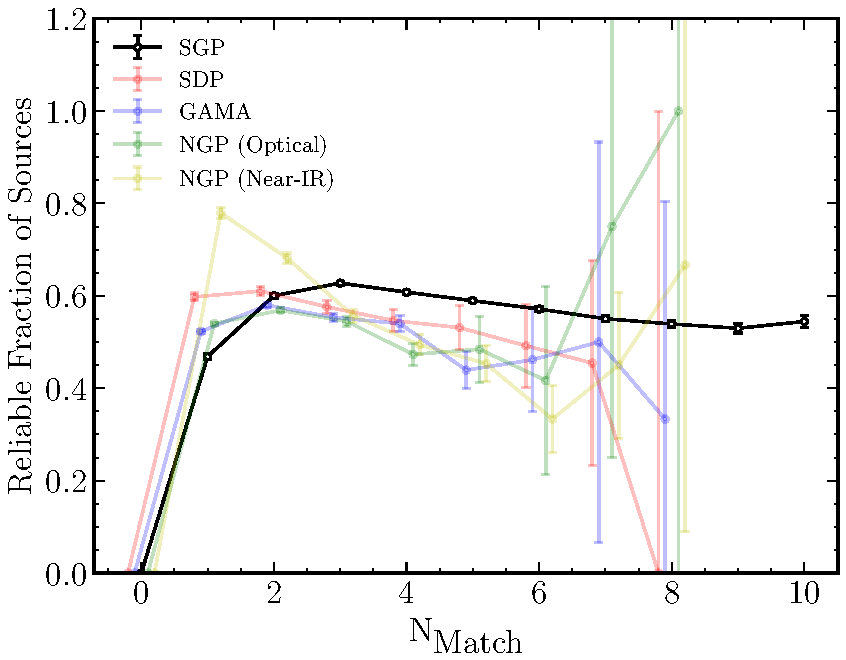
\includegraphics[width=\columnwidth]{Figures/multiplicity.pdf}
    \caption{The fraction of \textit{Herschel} sources with reliably matched counterparts as a function of the number of observed candidates. The results from various H-ATLAS fields are shown as the following lines: SGP (black, this work); SDP (red, \citealt{Smith_2011}); Phase 1 GAMA9 Field (blue, \citealt{Fleuren_2012}), GAMA (green, \citealt{Bourne_2016}), NGP (optical in yellow, near-IR in pink, \citealt{Furlanetto_2018}). All other works used a maximum search radius of 10" while the SGP analysis used 15". For clarity each line has been offset in $N_{\textrm{Match}}$ by a different value.}
    \label{fig:multiplicity}
\end{figure}

We can estimate the number of sources that have multiple genuine associations that were missed by the LR method by assuming that all candidates are associated with a single source if their combined reliabilities is greater than 0.8, but are missed because no individual counterpart meets the threshold. I find [...]\todo[color=orange]{Do calculation} such sources, however, due to the increased maximum $r$ and consequently increased average number of candidates per source, even moderately valued $R$ counterparts combine to exceed the reliability cut. Alternatively, we could use the likelihood values, $L$, for each counterpart, rather than their reliability as the likelihood has no upper limit unlike the bounds on reliability, $R \in [0, 1]$. From Equation \ref{eq:reliability_multiple_counterparts} a reliability of 0.8 or greater corresponds to $L > 0.66$, assuming a single candidate and a value of $Q = 0.835$. An estimate for the number of lost sources with multiple associated counterparts can be made assuming that a source with a best matched counterpart with $L > 0.66$ but $R < 0.8$ is influenced by nearby candidates. I find 33,967 sources that satisfy these conditions. However, this is likely an overestimate of the true number as a large fraction of these IDs will be due to a mixture of true mergers or close groups and chance alignments; a measure for the probability that two or more counterparts are physically associated is required to potentially identify galaxy groups or mergers.

An improved estimate that removes chance alignments can be made considering the photometric redshifts of the VIKING objects (the method of obtaining photometric redshifts for the VIKING sample is presented in Section \ref{sec:phot_z_VIKING}). As shown in \citealt{Fleuren_2012}, chance matches along the line of sight can be ruled out by comparing the redshifts of all possible matches, and considering them to be associated if they fall within $\sim$ 10\% of each other for photometric redshifts or $\sim$ 5\% if using spectroscopic redshifts. While this is a simple and effective method, it does not rule out sources that happen to lie on a similar line of sight to unrelated groups or mergers of galaxies (and the true ID remaining unmatched or beyond the VIKING survey limit). In the following, I describe a new method in which we use the background distribution of VIKING sources (as used for estimating the magnitude distribution of true counterparts in Section \ref{sec:true_counterparts_distribution}) to estimate the probability that a pair of VIKING galaxies with similar redshifts are associated with the sub-mm source. 

Firstly, I restrict both the SGP and background catalogues to contain only sources with two or more counterparts and I restrict this further to counterparts found within 8", as this is where the majority of $L > 0.66$ counterparts are found, reducing the chance of selecting pairs of galaxies that are unrelated to the source. For each position in both catalogues, I identify the pair of galaxies with the closest redshifts and calculate the difference in their redshifts divided by the error in the difference, i.e. $\Delta z/\sigma_{\Delta z}$. In Figure \ref{fig:delta_z_multiplicity} I show the probability distribution functions (PDFs) of $\Delta z/\sigma_{\Delta z}$ for the SGP catalogue (red line) and the background catalogue (black line). When a background subtraction of the SGP catalogue is made, we observe an excess close to $\Delta z = 0$ (blue line) where the area of this peak represents the probability that a close pair of VIKING galaxies is indeed related to the SPIRE source. I fit a Gaussian profile to the excess and calculate this probability to be 2 -- 5\% depending on the size of the bins used to generate the PDFs. By multiplying this probability by the total number of SPIRE sources for which we observe a close pair of VIKING galaxies, in this case we take this to be the width of the peak, $-0.1 \lesssim \Delta z/\sigma_{\Delta z} \gtrsim 0.1$, I find an estimate for the number of \textit{Herschel} sources with genuine multiple counterparts of $\sim$ 400 -- 1,000.

\begin{figure}
    \centering
    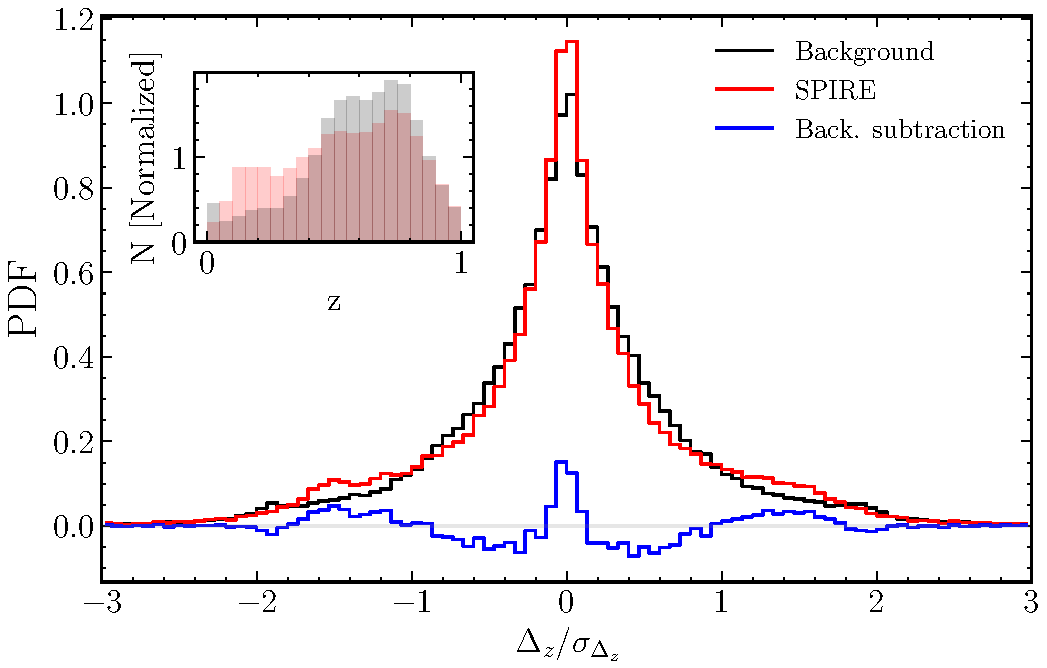
\includegraphics[width=\columnwidth]{Figures/delta_z_multiplicity.pdf}
    \caption{Probability distribution functions of $\Delta z/\sigma_{\Delta z}$, the difference between photometric redshifts of VIKING counterparts divided by the error in their difference, for pairs of galaxies located near 250\,\micron positions (within 8") in the SGP catalogue (red histogram) and near randomly located positions (black histogram). The blue histogram represents a background subtraction of the former. The excess located at $\Delta z = 0$ represents the subset of VIKING galaxy pairs with similar redshifts that are associated with the SPIRE source. The inset figure shows the normalized redshift distribution of VIKING counterparts observed within 8" of 250\,\micron positions in red and random positions in grey.}
    \label{fig:delta_z_multiplicity}
\end{figure}

It should be noted that this method is independent of the LR method and the resulting reliability values, and so the pair of VIKING objects chosen for each source does not always contain the candidate with the highest reliability. In total there are 70,880 sources where we observe two or more candidates with estimated photometric redshifts (within 8" of the source), of which approximately three quarters have best counterparts that are also part of the "redshift pair". The selected pairs for the remaining quarter of sources may be the locations of unassociated galaxy interactions or multiple systems related to the sub-mm source that is overlooked by the one-to-one matching of the LR method. The subset used here is approximately one third of all sources in the SGP (70,880/193,527) and so we expect mant more galaxy interactions and groups to be in the full SGP catalogue. We also note that the fraction accounting for all sources may be higher as there is evidence to suggest that the merger rate of galaxies evolves with redshift and reaches a peak at $z \sim 1.2$ (e.g. \citealt{Bell_2006}; \citealt{Ryan_2008}). If this is true, then a large fraction of interacting systems may be those beyond the VIKING detection limit and therefore lie in the blank SPIRE fields.

\subsection{Photometric Redshifts of Submillimeter Sources}
\label{sec:phot_z_Herschel}

Any study on the evolution of fundamental properties of extragalactic sources requires an estimate for the age of the galaxy and therefore its redshift. Having crossmatched the sources detected on the sub-mm images with the sources on the VIKING images, we can begin to construct spectral energy distributions (SEDs) that places constraints on the stellar properties as well as the dust emission. 

The dust emission can be well approximated using a two-temperature modified blackbody model (see Section [...]\todo[color=green]{Add reference to blackbody functions when written} for a more detailed description on modified blackbody functions). A characteristic SED that can be used to approximate the SED of a typical H-ATLAS source is presented in \citealt{Pearson_2013} and takes the form:

\begin{equation}
    S_\nu = A[B_\nu(T_{\textrm{hot}})\nu^\beta + \alpha B_\nu(T_{\textrm{cold}})\nu^\beta],
\label{eq:pearson_sed_model}
\end{equation}

where $S_\nu$ is the flux density of the source at the rest frame frequency, $\nu$, $A$ is a normalization factor, $B(T)$ represents the Planck function at temperature $T$, of which we assume two dust temperatures, $T_{\textrm{hot}}$ and $T_{\textrm{cold}}$, $\beta$ is the dust emissivity index and $\alpha$ represents the fraction of cold dust mass to hot dust mass. Using a sample of 40 H-ATLAS sources with spectroscopic redshifts, the optimal set of parameters were measured to be $T_{\textrm{hot}} = 46.9$\,K, $T_{\textrm{cold}} = 23.9$\,K and $\alpha = 30.1$ (assuming a fixed $\beta = 2$). This leaves a model with only two free parameters, the normalization and the redshift; a necessary simplification given that each source had at most three flux densities at the central wavelengths of the SPIRE bands (the PACS 100 and 160\,\micron flux densities were not included as the \textit{Herschel} images are less sensitive at these wavelengths). For each source the normalization and redshift were varied until a minimum chi squared was reached:

\begin{equation}
    \chi^2 = \sum_i \frac{S_i - S_{i,m}}{E_i^2},
\end{equation}

where $S_i$ is the flux density at each SPIRE wavelength, $i$, $S_{i,m}$ is the model prediction of the flux and $E_i$ is the error on the flux at wavelength $i$. 

While all sources in the SGP have estiamtes for their flux and flux errors at the SPIRE wavelengths in the second data release, the errors do not account for calibration errors.

\subsection{Photometric Redshifts of VIKING Counterparts}
\label{sec:phot_z_VIKING}

%\subsection{Comparison between H-ATLAS Data Releases}
% Include correlations with redshift now they have been described (e.g. flux and magnitude against redshift)
% Include a description of the full H-ATLAS: a legacy product that has no plans for being replaced
%\section{Gravitational Lensing in the SGP}
%\subsection{The Brightest Lenses}
%\subsection{Extending the Search for Lenses to Lower Fluxes}
\listoftodos

\chapter{Conclusion}
\label{chapter:Conclusion}
\chapquote{``A quote"}{By whom}{From what source}

\section{Thesis Overview}
\section{Key Results}
\section{Future work}
\section{Concluding remarks}

\appendix


\titleformat{\chapter}[display]{}{}{0pt}{{\textbf \huge \textsc{Appendix} \thechapter}\\ \huge \textbf \textsc}[\titlerule\vspace{2pt}\titlerule]

\chapter{Candidate Lensed Sources in the SGP ($S_{\textrm{500\,\micron}}$ > 100\,mJy)}



% Define bibliography
\titleformat{\chapter}[display]{}{}{0pt}{\huge \textbf \textsc}[\titlerule\vspace{2pt}\titlerule]
%\input{journalCommand}


%\printbibliography
\bibliographystyle{mnras}
\bibliography{Thesis.bib}

%% Uncomment \layout* to view layout config page
% \layout*
\end{document}